%% thesis.tex — Main driver for SEKD thesis manuscript
%% Adaptive Retrieval Planning for Enterprise Knowledge Management:
%% A Controlled Evaluation on the Synthetic Enterprise Knowledge Dataset (SEKD)
%%
%% Author: Pingu / Information Systems Capstone Design
%% Date: June 2026
%% Compile: pdflatex thesis.tex && bibtex thesis && pdflatex thesis.tex && pdflatex thesis.tex

\documentclass[12pt, a4paper, twoside]{report}

%% ────────────── Encoding & Fonts ──────────────
\usepackage[T1]{fontenc}
\usepackage[utf8]{inputenc}
\usepackage{lmodern}
\usepackage{microtype}

%% ────────────── Page Layout ──────────────
\usepackage[
  a4paper,
  top=30mm,
  bottom=30mm,
  inner=35mm,
  outer=25mm,
  headheight=15pt
]{geometry}
\usepackage{fancyhdr}
\pagestyle{fancy}
\fancyhf{}
\fancyhead[LE,RO]{\thepage}
\fancyhead[LO]{\nouppercase{\rightmark}}
\fancyhead[RE]{\nouppercase{\leftmark}}
\renewcommand{\headrulewidth}{0.4pt}

%% ────────────── Math & Symbols ──────────────
\usepackage{amsmath}
\usepackage{amssymb}
\usepackage{bm}

%% ────────────── Tables ──────────────
\usepackage{booktabs}
\usepackage{multirow}
\usepackage{multicol}
\usepackage{array}
\usepackage{tabularx}
\usepackage{siunitx}
\sisetup{group-separator={,}, group-minimum-digits=4}

%% ────────────── Figures ──────────────
\usepackage{graphicx}
\usepackage{float}
\usepackage{caption}
\usepackage{subcaption}
\captionsetup{font=small, labelfont=bf}

%% ────────────── Colors ──────────────
\usepackage[dvipsnames]{xcolor}

%% ────────────── Hyperlinks ──────────────
\usepackage[
  colorlinks=true,
  linkcolor=NavyBlue,
  citecolor=OliveGreen,
  urlcolor=MidnightBlue,
  pdfauthor={Won Young Shin},
  pdftitle={Adaptive Retrieval Planning for Enterprise Knowledge Management},
  pdfsubject={Information Systems, Retrieval-Augmented Generation, Enterprise Search},
  pdfkeywords={BM25, Dense Retrieval, Hybrid RRF, Adaptive Planning, GPT-5, Enterprise RAG, Agentic RAG, LangGraph, Re-retrieval}
]{hyperref}

%% ────────────── Code Listings ──────────────
\usepackage{listings}
\lstset{
  basicstyle=\ttfamily\footnotesize,
  breaklines=true,
  frame=single,
  numbers=left,
  numberstyle=\tiny,
  keywordstyle=\color{NavyBlue}\bfseries,
  commentstyle=\color{OliveGreen},
  stringstyle=\color{BrickRed}
}

%% ────────────── Bibliography ──────────────
\usepackage[round,authoryear]{natbib}
\bibliographystyle{plainnat}

%% ────────────── Misc Formatting ──────────────
\usepackage{setspace}
\onehalfspacing
\usepackage{enumitem}
\setlist[description]{leftmargin=2em, labelindent=0em, style=nextline}
\usepackage{placeins}  % \FloatBarrier to prevent figures drifting past sections
\clubpenalty=10000     % suppress orphan lines
\widowpenalty=10000    % suppress widow lines
\microtypesetup{activate={true,nocompatibility}}  % suppress setspace/microtype warning

%% ────────────── Chapter Title Style ──────────────
\usepackage{titlesec}
\titleformat{\chapter}[display]
  {\normalfont\huge\bfseries}
  {\chaptertitlename\ \thechapter}
  {20pt}
  {\Huge}
\titlespacing*{\chapter}{0pt}{30pt}{20pt}

%% ────────────── Abstract Environment ──────────────
\renewenvironment{abstract}{
  \cleardoublepage
  \chapter*{Abstract}
  \addcontentsline{toc}{chapter}{Abstract}
}{}

%% ────────────── Figure Path ──────────────
\graphicspath{{../final_report/figures/}}

%% ─────────────────────────────────────────────────────────────────────────────
\begin{document}

%% ────────────── Title Page ──────────────
\begin{titlepage}
\centering
\vspace*{2cm}

{\Large\textbf{Hanyang University}}\\[0.5em]
{\large Department of Information Systems}\\[3em]

\rule{\textwidth}{1.5pt}\\[0.5em]
{\huge\bfseries Adaptive Retrieval Planning for\\[0.3em]
Enterprise Knowledge Management:\\[0.3em]
A Controlled Evaluation on the\\[0.3em]
Synthetic Enterprise Knowledge Dataset}\\[0.5em]
\rule{\textwidth}{1.5pt}\\[3em]

{\large Capstone Design Thesis}\\[2em]

{\large\bfseries Won Young Shin}\\[0.3em]
{\large Information System Capstone Design}\\[1em]
{\large pingu090@hanyang.ac.kr}\\[4em]

\vfill

{\large June 2026}\\[1em]

{\normalsize
Submitted in partial fulfilment of the requirements for the\\
Bachelor of Science in Information Systems\\[1em]
Supervisor: Prof. Ook Lee
}

\end{titlepage}

%% ────────────── Front Matter ──────────────
\pagenumbering{roman}

%% abstract.tex
\begin{abstract}

Enterprise knowledge management systems increasingly rely on Retrieval-Augmented Generation (RAG) to surface relevant information from large, heterogeneous document corpora. A critical but underexplored design decision in such systems is \emph{retrieval strategy selection}: given a user query, should the system apply sparse keyword retrieval, dense semantic retrieval, or a hybrid fusion of both? This thesis investigates \emph{adaptive retrieval planning} — the automated selection of a retrieval strategy based on query characteristics — as a mechanism for improving retrieval quality in enterprise knowledge management contexts.

We conduct a controlled evaluation on the Synthetic Enterprise Knowledge Dataset (SEKD), a purpose-built corpus of 120 enterprise documents spanning six categories (API Documentation, HR Policies, Project Meeting Notes, Security Policies, System Design Documents, and Travel Policies), segmented into 1,206 section-aware chunks, with 405 annotated queries covering six reasoning types (single-hop, multi-hop, aggregation, comparison, exception, and temporal). We evaluate five systems along a complexity-cost axis: BM25 (sparse), BGE-small-en-v1.5 dense retrieval, Hybrid Reciprocal Rank Fusion (RRF), a seven-rule deterministic planner, and a GPT-5-based zero-shot planner using a structured prompt.

Our experiments address seven research questions spanning retrieval architecture selection, category- and reasoning-type-level performance variation, and the relative effectiveness of rule-based versus LLM-based adaptive planning. Key findings are: (1) Hybrid RRF outperforms both unimodal methods on most metrics (MRR: +15.8\% over BM25, +5.6\% over Dense), confirming lexical and semantic signals are complementary; (2) the seven-rule planner achieves the highest Recall@10 (0.755) and Hit@10 (0.808) of any system at zero operational cost; (3) GPT-5 achieves the highest MRR (0.533) and nDCG@10 (0.570) but does not outperform the rule planner on Strategy Selection Accuracy (77.6\% vs.\ 78.4\%) and costs \$6.18 for 380 queries; (4) exception clause and temporal queries are universal failure modes across all evaluated systems, with Dense achieving zero recall on temporal queries and no system exceeding Recall@10 = 0.412 on exception queries.

These findings suggest that adaptive retrieval planning provides measurable but modest improvements over fixed-strategy retrieval, that deterministic planning is competitive with LLM-based planning at orders-of-magnitude lower cost, and that the primary remaining challenge for enterprise RAG is specialized handling of exception and temporal query patterns.

\bigskip
\noindent\textbf{Keywords:} Retrieval-Augmented Generation, Enterprise Search, Adaptive Retrieval, BM25, Dense Retrieval, Hybrid Retrieval, Reciprocal Rank Fusion, Large Language Models, Query Planning, Information Retrieval Evaluation

\end{abstract}


\clearpage
\tableofcontents

\clearpage
\listoffigures
\addcontentsline{toc}{chapter}{List of Figures}

\clearpage
\listoftables
\addcontentsline{toc}{chapter}{List of Tables}

%% ────────────── Acronym / Notation ──────────────
\clearpage
\chapter*{Notation and Abbreviations}
\addcontentsline{toc}{chapter}{Notation and Abbreviations}

\begin{tabular}{ll}
\toprule
\textbf{Abbreviation} & \textbf{Meaning} \\
\midrule
AA      & Answer Agent \\
ANN     & Approximate Nearest Neighbor \\
API     & Application Programming Interface \\
BM25    & Best Match 25 (Okapi BM25 retrieval function) \\
Dense   & Dense embedding-based retrieval \\
DPR     & Dense Passage Retrieval \\
EMNLP  & Conference on Empirical Methods in NLP \\
HR      & Human Resources \\
IR      & Information Retrieval \\
LLM     & Large Language Model \\
MCP     & Model Context Protocol \\
MRR     & Mean Reciprocal Rank \\
nDCG    & Normalized Discounted Cumulative Gain \\
PA      & Planning Agent \\
QAA     & Query Analysis Agent \\
RA      & Retrieval Agent \\
RAG     & Retrieval-Augmented Generation \\
RRF     & Reciprocal Rank Fusion \\
SEKD    & Synthetic Enterprise Knowledge Dataset \\
SSA     & Strategy Selection Accuracy \\
TF-IDF  & Term Frequency–Inverse Document Frequency \\
VA      & Validation Agent \\
\bottomrule
\end{tabular}

%% ────────────── Main Matter ──────────────
\pagenumbering{arabic}

%% introduction.tex
\chapter{Introduction}
\label{chap:introduction}

\section{Motivation}
\label{sec:intro_motivation}

Modern enterprises generate and maintain vast quantities of structured and semi-structured knowledge: technical API references, HR policy manuals, architectural design documents, meeting minutes, security compliance guides, and operational travel policies. As these corpora grow in volume and heterogeneity, the challenge of locating relevant information efficiently becomes a first-order organizational problem. Employees searching across hundreds of policy documents, engineers querying system design archives, and automated agents performing compliance checks all require retrieval systems that surface the right information reliably and quickly.

Retrieval-Augmented Generation (RAG) has emerged as a leading paradigm for knowledge-intensive natural language processing \citep{lewis2020rag}. A RAG system retrieves a set of candidate documents or passages from a corpus and conditions a generative language model's output on those retrieved passages. The retrieval step is therefore the critical upstream dependency: if relevant documents are not retrieved, no amount of downstream generation quality can compensate. The quality of retrieval is measured along two primary dimensions --- \emph{coverage} (does the system find all relevant documents?) and \emph{ranking quality} (does it place the most relevant documents highest?).

Enterprise corpora present distinctive challenges for standard retrieval methods. Unlike web search or open-domain question answering, enterprise queries span a wide range of reasoning types --- from simple single-hop factual lookups to complex multi-hop reasoning across multiple documents, temporal ordering queries, policy exception clause extraction, and multi-attribute aggregation tasks. Different reasoning types benefit from different retrieval signals: temporal queries require exact date-token matching that dense embeddings cannot capture; exception clause queries require semantic identification of negation and conditional language; multi-hop queries benefit from broad document coverage. No single retrieval method is optimal across this full distribution of enterprise query types.

\emph{Adaptive retrieval planning} addresses this challenge by dynamically selecting the retrieval strategy best suited to each incoming query, rather than applying a single fixed strategy to all queries. A retrieval planner examines query characteristics --- its reasoning type, semantic content, named entities, or difficulty factors --- and routes the query to the most appropriate retrieval backend. This routing decision has the potential to improve retrieval quality at minimal computational overhead, provided the planner's strategy selection aligns with the empirically optimal strategy for each query type.

This thesis investigates adaptive retrieval planning in the enterprise knowledge management context. We ask: can a retrieval planner --- either a lightweight deterministic rule system or a large language model --- outperform the best fixed-strategy retrieval baseline, and at what cost? We evaluate both planning paradigms on a controlled, fully annotated enterprise corpus and measure their performance against seven pre-defined research questions.

\section{Problem Statement}
\label{sec:intro_problem}

This thesis addresses the following core problem:

\begin{quote}
\textit{Given a heterogeneous enterprise knowledge corpus containing documents of multiple types and a set of queries spanning diverse reasoning types, what is the most effective and cost-efficient retrieval strategy selection mechanism, and to what extent does adaptive retrieval planning improve over fixed-strategy retrieval baselines?}
\end{quote}

We decompose this problem into three sub-problems:

\begin{enumerate}
    \item \textbf{Retrieval baseline selection}: Among BM25 (sparse), dense embedding retrieval, and Hybrid Reciprocal Rank Fusion, which method performs best overall and by document category and query reasoning type?
    \item \textbf{Rule-based adaptive planning}: Can a small set of deterministic rules mapping query metadata to retrieval strategies outperform the best fixed-strategy baseline on enterprise knowledge queries?
    \item \textbf{LLM-based adaptive planning}: Can a large language model (GPT-5) perform zero-shot retrieval strategy planning that surpasses both the fixed-strategy baseline and the rule-based planner, and is the resulting quality improvement cost-justified?
\end{enumerate}

\section{Research Questions}
\label{sec:intro_rqs}

We organize our investigation around seven research questions (RQ1--RQ7):

\begin{description}
    \item[RQ1] Does hybrid retrieval (BM25 + Dense) outperform single-method baselines on enterprise knowledge queries?
    \item[RQ2] Which retrieval method performs best across different enterprise document categories?
    \item[RQ3] How does retrieval performance vary across query reasoning types?
    \item[RQ4] Can a rule-based adaptive planner outperform fixed-strategy retrieval?
    \item[RQ5] Which LLM prompt strategy is optimal for retrieval planning?
    \item[RQ6] Does GPT-5 outperform the rule-based planner on Strategy Selection Accuracy?
    \item[RQ7] What are the primary failure modes of LLM-based retrieval planning?
\end{description}

RQ1--RQ3 establish the retrieval baseline landscape. RQ4 evaluates deterministic adaptive planning. RQ5--RQ7 evaluate LLM-based planning. Together, these questions span the full design space for retrieval strategy selection in enterprise knowledge management.

\subsection*{Extension: V2 Agentic RAG (RQ8--RQ13)}
\label{sec:intro_rqs_v2}

The V1 experiments reveal that all static planning approaches share a structural limitation: retrieval strategy selection is made once per query and cannot be corrected when the initial strategy fails. Two query types that proved consistently intractable under V1 --- exception handling (Recall@10 $\leq 0.412$) and temporal reasoning (Recall@10 $\leq 0.200$) --- motivate a fundamentally different architecture. Chapters~\ref{chap:v2_methodology}--\ref{chap:v2_results} introduce the V2 Agentic RAG pipeline, which wraps the V1 retrieval infrastructure in a LangGraph state machine that supports iterative re-retrieval conditioned on a learned validation signal. Six additional research questions govern this extension:

\begin{description}
    \item[RQ8]  Does the V2 agentic pipeline outperform the best V1 planner (Rule Planner, Recall@10$={0.755}$) on overall retrieval quality?
    \item[RQ9]  What is the contribution of the iterative re-retrieval loop over a single-pass agentic baseline?
    \item[RQ10] Does signal-matched (adaptive) validation scoring outperform rank-order scoring for retrieval validation?
    \item[RQ11] How much does oracle query analysis contribute to V2 performance compared with heuristic LLM-based query analysis?
    \item[RQ12] Does the targeted re-retrieval mechanism specifically address the exception and temporal query failure modes identified in V1?
    \item[RQ13] What are the primary failure modes of the V2 agentic pipeline after all re-retrieval loops are exhausted?
\end{description}

\section{Research Contributions}
\label{sec:intro_contributions}

This thesis makes the following contributions:

\textbf{Methodological}: We construct the Synthetic Enterprise Knowledge Dataset (SEKD), a fully annotated enterprise corpus comprising 120 documents across 6 categories, 1,206 section-aware chunks, and 405 queries with ground-truth answer chunks and oracle retrieval strategy labels. SEKD supports controlled, reproducible evaluation of retrieval and planning methods and is made available for future research.

\textbf{Empirical}: We report the first systematic comparison of BM25, dense retrieval, Hybrid RRF, rule-based planning, LLM-based planning, and agentic re-retrieval on a controlled enterprise knowledge corpus. Our results quantify the performance contribution of each architectural layer and identify the specific query types where each method excels or fails.

\textbf{Practical}: We demonstrate that a seven-rule deterministic planner achieves the highest Recall@10 (0.755) among V1 systems at zero operational cost, and that GPT-5-based planning provides ranking quality advantages (MRR: +2.0\%) that may justify LLM planning costs in precision-critical enterprise applications. The V2 agentic extension provides an iterative correction mechanism for the exception and temporal query types that are intractable under all V1 approaches.

\textbf{Analytical}: We characterize the primary failure modes of LLM-based retrieval planning --- category confusion on fine-grained single-hop queries (55.3\% of errors) and systematic temporal query mis-routing (0\% Strategy Selection Accuracy) --- and identify the structural causes of exception and temporal query failure across all evaluated retrieval methods. The V2 pipeline's failure mode taxonomy (Section~\ref{sec:v2_pipeline_stats}) extends this analysis to the agentic setting.

\textbf{Systems}: We implement and release the V2 Agentic RAG system as a fully operational LangGraph pipeline, comprising five specialised agents and a structured evaluation harness. The implementation serves as a reproducible foundation for future work on iterative enterprise retrieval.

\section{Thesis Structure}
\label{sec:intro_structure}

The remainder of this thesis is organized as follows. Chapter~\ref{chap:litreview} reviews related work in information retrieval, dense retrieval, hybrid fusion methods, and LLM-augmented systems. Chapter~\ref{chap:methodology} describes the SEKD corpus construction, retrieval system designs, planner architectures, and evaluation framework. Chapter~\ref{chap:results} presents the experimental results for all five V1 systems. Chapter~\ref{chap:discussion} discusses why each V1 system performed as it did and draws implications for enterprise RAG design. Chapter~\ref{chap:conclusion} summarizes the V1 principal findings. Chapter~\ref{chap:v2_methodology} introduces the V2 Agentic RAG pipeline architecture and evaluation design. Chapter~\ref{chap:v2_results} presents the V2 evaluation results addressing RQ8--RQ13.

%% literature_review.tex
\chapter{Related Work}
\label{chap:litreview}

\section{Information Retrieval Foundations}
\label{sec:lit_ir}

Information retrieval (IR) is the study of systems that retrieve material in response to an information need \citep{manning2008ir}. The canonical retrieval pipeline consists of indexing a document collection and, at query time, scoring each indexed document against the query to produce a ranked list. Modern enterprise retrieval systems inherit decades of IR research, particularly on sparse term-weighting and dense representation learning.

\subsection{Sparse Retrieval: BM25}
The Best Match 25 (BM25) retrieval function \citep{robertson1995okapi,robertson2009bm25} is the dominant sparse retrieval method in production systems. BM25 extends the classic TF-IDF weighting scheme with term frequency saturation (parameter $k_1$) and document length normalization (parameter $b$), computing a relevance score between a query $q$ and document $d$ as:
\begin{equation}
    \text{BM25}(d, q) = \sum_{t \in q} \text{IDF}(t) \cdot \frac{f(t,d) \cdot (k_1 + 1)}{f(t,d) + k_1 \cdot (1 - b + b \cdot \frac{|d|}{\text{avgdl}})}
    \label{eq:bm25}
\end{equation}
where $f(t,d)$ is the term frequency of $t$ in $d$, $|d|$ is document length, and $\text{avgdl}$ is the average document length in the corpus. BM25 is computationally efficient via inverted index lookup, interpretable, and strong on exact-match queries involving named entities, version numbers, and policy codes. Its primary weakness is vocabulary mismatch: queries and documents that discuss the same concept using different vocabulary receive low BM25 scores.

For enterprise corpora with both structured (policy codes, API endpoints) and unstructured (conceptual descriptions, meeting minutes) content, BM25's strengths and weaknesses are both highly relevant \citep{robertson2004understanding}. Queries involving exact identifiers benefit from BM25's precise token matching, while semantic queries about concepts or policies may suffer from vocabulary mismatch.

\subsection{Dense Retrieval}
Dense retrieval represents queries and documents as dense vectors in a continuous embedding space, computing relevance as vector similarity \citep{karpukhin2020dpr}. The Dense Passage Retrieval (DPR) model demonstrated that bi-encoder architectures trained on question-answer pairs could substantially outperform BM25 on open-domain question answering, particularly for queries where the answer was paraphrased rather than lexically identical to the query.

Modern dense retrieval systems use pre-trained transformer encoders fine-tuned for retrieval tasks. The BAAI General Embedding series \citep{xiao2023bge} provides lightweight, high-quality encoders that achieve strong retrieval performance across diverse domains. The BGE-small-en-v1.5 model used in this study encodes text into 384-dimensional vectors and supports cosine similarity-based retrieval via approximate nearest-neighbor (ANN) indices. Dense models encode semantic relationships that BM25 cannot capture --- synonymy, paraphrase, and conceptual similarity --- making them particularly effective for comparison and single-hop semantic queries.

However, dense retrieval has known failure modes. Static dense embeddings trained on general text corpora do not encode temporal ordering signals such as date sequences or version histories \citep{manning2008ir}. They also struggle with rare entities and exact string matching for specialized technical terms, where the embedding space may conflate semantically similar but functionally distinct concepts. For enterprise corpora with strong temporal or version-dependent content, these limitations are consequential.

ColBERT \citep{khattab2020colbert} and SPLADE \citep{formal2021splade} represent hybrid sparse-dense approaches that aim to combine the complementary strengths of lexical and semantic matching within a single model. While these methods outperform both BM25 and bi-encoder dense retrieval on some benchmarks, they require specialized training and index structures not available for arbitrary domain-specific corpora.

\subsection{Hybrid Retrieval and Reciprocal Rank Fusion}

Given the complementarity of sparse and dense signals, hybrid retrieval systems that combine both methods have become widely adopted in enterprise search \citep{luan2021sparse_dense}. The Reciprocal Rank Fusion (RRF) algorithm \citep{cormack2009rrf} provides a simple, parameter-light method for combining ranked lists from multiple retrieval systems:
\begin{equation}
    \text{RRF}(d) = \sum_{r \in R} \frac{1}{k + r(d)}
    \label{eq:rrf}
\end{equation}
where $R$ is the set of ranked lists, $r(d)$ is the rank of document $d$ in list $r$, and $k$ is a constant (typically 60 in the original formulation; we use $k=10$ following TREC practices). RRF has been shown to outperform individual rank learning methods and Condorcet voting on standard IR benchmarks \citep{cormack2009rrf}.

The BEIR benchmark \citep{thakur2021beir} provides evidence that hybrid retrieval is robust across heterogeneous retrieval tasks including biomedical, legal, and general web search domains. This generalization motivates the application of Hybrid RRF to enterprise knowledge retrieval, where query distributions are similarly heterogeneous.

\section{Retrieval-Augmented Generation}
\label{sec:lit_rag}

Retrieval-Augmented Generation (RAG) \citep{lewis2020rag} conditions a language model's generative output on retrieved passages, allowing the model to access domain-specific or up-to-date information not encoded in its parameters. The RAG architecture consists of: (1) a retriever that maps a query to a set of passages, and (2) a reader/generator that conditions on the query and retrieved passages to produce an answer.

Subsequent work has extended the original RAG formulation in multiple directions. Fusion-in-Decoder (FiD) \citep{izacard2021fid} processes each retrieved passage independently and fuses their representations in the decoder, enabling the use of larger retrieval sets. RETRO \citep{borgeaud2022retro} integrates retrieval into the pretraining process, enabling trillion-token-scale knowledge retrieval. Self-RAG \citep{asai2023selfrag} augments the generator with learned reflection tokens that allow it to decide when to retrieve and how to evaluate retrieved passages.

Active retrieval augmented generation \citep{jiang2023active} addresses multi-step reasoning scenarios where a single retrieval step may be insufficient: the system interleaves generation and retrieval, issuing new retrieval queries based on intermediate generation outputs. This approach is most relevant for multi-hop queries where answering requires synthesizing evidence from multiple documents retrieved in sequence.

\section{Query Classification and Adaptive Retrieval}
\label{sec:lit_adaptive}

Query classification is the task of assigning an incoming query to one of a predefined set of categories or difficulty classes based on query features. In classical IR, query classification has been applied to route queries to specialized search backends (e.g., entity queries to structured databases, web queries to document indexes) or to select query expansion strategies \citep{baeza1999modern}. In the RAG context, query classification enables \emph{adaptive retrieval}: selecting the retrieval strategy most likely to return high-quality results for the given query.

Domain-matched pretraining and fine-tuning have been shown to substantially improve dense retrieval performance for specialized corpora \citep{oguz2021domain}. However, fine-tuning is expensive and requires labeled data. A simpler alternative is to classify queries based on their structural features (query length, presence of named entities, detected reasoning type) and apply deterministic routing rules. This approach is analogous to rule-based expert systems and avoids the computational overhead of model-based classification.

LLM-based query planning builds on the success of chain-of-thought prompting \citep{wei2022chain} and tool use \citep{schick2023toolformer,yao2023react} to enable language models to decompose complex queries, select retrieval strategies, and issue targeted retrieval requests. WebGPT \citep{nakano2022webgpt} demonstrated that language models can be trained to use web search tools effectively. Toolformer \citep{schick2023toolformer} showed that models can self-supervise tool use from examples. ReAct \citep{yao2023react} integrates reasoning traces and action execution in an interleaved manner, enabling multi-step retrieval-augmented reasoning.

Query rewriting \citep{ma2023query_rewrite} is a related technique that rephrases queries to improve retrieval quality without changing the retrieval strategy. Rewriting can reduce vocabulary mismatch for BM25 and improve the semantic alignment of queries with dense encoder training distributions.

\section{LLM-Based Planning and Augmented Language Models}
\label{sec:lit_llm_planning}

The augmented language model survey \citep{mialon2023augmented} identifies retrieval, tool use, and reasoning as the three primary augmentation dimensions for language models. Retrieval augmentation provides factual grounding; tool use extends the model's action space; reasoning augmentation (chain-of-thought, scratchpad, self-reflection) improves compositional problem-solving.

Large language models have demonstrated strong zero-shot performance on structured classification tasks when provided with appropriate prompting \citep{wei2022chain}. The structured prompt approach \citep{mialon2023augmented} provides explicit metadata about the classification task in the prompt, enabling the model to apply decision logic without requiring in-context examples. This is directly analogous to the structured retrieval planning prompt evaluated in this thesis, which provides the model with the query's reasoning type, difficulty factors, and document category.

However, LLMs have known failure modes on tasks that require precise logical rules. Shi et al. \citep{shi2023large} show that LLMs are easily distracted by irrelevant context, and that performance on reasoning tasks degrades when the problem framing includes confounding information. This is relevant to the retrieval planning context, where the optimal strategy for a query depends on specific, non-obvious features (e.g., the presence of exact identifiers suggesting BM25 routing) that may be overridden by the model's learned priors.

GPT-5 is an extended reasoning model that uses internal chain-of-thought computation (``reasoning tokens'') before producing its visible output. This architecture requires careful configuration of the \texttt{max\_completion\_tokens} parameter, which provides a shared budget for both reasoning tokens and visible output tokens. Insufficient budget allocation causes the model to exhaust its reasoning budget before producing output, resulting in empty responses --- a failure mode specific to reasoning models.

\section{Evaluation of Retrieval Systems}
\label{sec:lit_eval}

Standard IR evaluation metrics include Recall@$k$ (fraction of relevant documents found in the top-$k$ ranked results), Mean Reciprocal Rank (MRR; reciprocal of the rank of the first relevant result), normalized Discounted Cumulative Gain (nDCG; position-discounted gain normalized by ideal ranking), and Hit Rate@$k$ (binary indicator of at least one relevant document in top-$k$) \citep{manning2008ir,jaervelin2002ndcg}.

The Text Retrieval Conference (TREC) \citep{voorhees2005trec} has been the primary driver of standardized IR evaluation since 1992, establishing the pooling and relevance judgment methodology used in large-scale retrieval benchmarks. The BEIR benchmark \citep{thakur2021beir} extends this tradition to dense and hybrid retrieval evaluation across 18 diverse datasets.

For enterprise retrieval evaluation, the key evaluation challenge is ground-truth construction: identifying the complete set of relevant documents for each query requires human annotation or semi-automated construction from structured documents. The SEKD corpus used in this thesis employs a programmatic ground-truth construction approach, using the query generation process to embed evidence chunk identifiers in each query's metadata, enabling exact-match ground-truth evaluation without human annotation.

\section{Summary}
\label{sec:lit_summary}

The literature establishes that: (1) BM25 and dense retrieval are complementary rather than competing methods; (2) Hybrid RRF is a well-motivated and broadly validated approach to combining their signals; (3) adaptive retrieval planning is theoretically motivated but empirically understudied for enterprise corpora; and (4) LLM-based planning offers potential advantages on semantically complex queries but has known failure modes on tasks requiring precise logical rules.

This thesis provides the first controlled empirical comparison of all five approaches (BM25, Dense, Hybrid, Rule Planner, LLM Planner) on a purpose-built enterprise knowledge corpus, addressing the gap between the theoretical motivation for adaptive retrieval planning and its empirical validation in enterprise settings.

%% methodology.tex
\chapter{Methodology}
\label{chap:methodology}

\section{Overview}
\label{sec:method_overview}

The experimental program consists of nine sequential phases, each building on artifacts produced by its predecessors. Phases 2--4 construct the evaluation corpus and query set. Phases 5--7 evaluate fixed retrieval baselines. Phase 8 evaluates the rule-based planner. Phase 9 evaluates the LLM-based planner. Phase 10 (this report) synthesizes all results.

\section{Dataset: The Synthetic Enterprise Knowledge Dataset (SEKD)}
\label{sec:method_dataset}

\subsection{Corpus Construction}

The Synthetic Enterprise Knowledge Dataset (SEKD) was designed to provide a controlled evaluation environment for enterprise retrieval methods. The corpus comprises 120 documents across six enterprise document categories, with 20 documents per category. Table~\ref{tab:dataset} provides complete corpus statistics.

\begin{description}
    \item[API Documentation] Technical reference documents for software APIs including endpoint descriptions, request/response schemas, authentication methods, and version changelogs.
    \item[HR Policies] Human resources policy documents including recruitment, compensation, leave, and performance management guidelines.
    \item[Project Meeting Notes] Structured meeting minutes including decisions, action items, attendees, and project progress summaries.
    \item[Security Policies] Enterprise security standards covering access control, incident response, data classification, and compliance requirements.
    \item[System Design Documents] Architectural design documents describing system components, integration patterns, capacity planning, and technical decisions.
    \item[Travel Policies] Corporate travel expense policies including booking procedures, reimbursement limits, and approval workflows.
\end{description}

Documents were generated using a Jinja2-based templating pipeline with Pydantic v2 domain models, producing syntactically varied, semantically coherent enterprise documents. Each document is structured with hierarchical sections and contains realistic entity references (project codes, version numbers, policy codes, dates) appropriate to its category.

\subsection{Chunking}

Documents were segmented using a section-aware chunking strategy that respects document section boundaries. The chunker produces 1,206 chunks in total, with complete metadata coverage including: \texttt{chunk\_id}, \texttt{document\_id}, \texttt{category}, \texttt{section\_title}, and \texttt{text}. Mean chunk length is approximately 220 tokens.

\subsection{Query Generation and Annotation}

The query set contains 405 queries: 380 answerable and 25 unanswerable. Queries were generated programmatically from document content using six reasoning types:

\begin{description}
    \item[single\_hop] ($n{=}220$, 57.9\%) Queries answerable from a single document section. The majority query type, reflecting direct information lookup.
    \item[multi\_hop] ($n{=}53$, 13.9\%) Queries requiring synthesis of evidence from multiple documents or sections.
    \item[aggregation] ($n{=}35$, 9.2\%) Queries requiring collection and summarization of information across multiple instances (e.g., ``list all API endpoints that require OAuth'').
    \item[comparison] ($n{=}33$, 8.7\%) Queries requiring comparison of two or more entities on specified attributes.
    \item[exception] ($n{=}34$, 8.9\%) Queries targeting exception clauses, conditional exclusions, or special-case policies within documents.
    \item[temporal] ($n{=}5$, 1.3\%) Queries requiring temporal ordering or date-based reasoning.
\end{description}

Each query includes ground-truth required chunk IDs derived from verbatim evidence spans in the source documents, enabling exact-match retrieval evaluation. A subset of queries include difficulty factor annotations: \texttt{table\_dependency}, \texttt{exception\_handling}, \texttt{temporal\_reasoning}, \texttt{document\_version\_conflict}, and \texttt{cross\_category}. Each query also carries an oracle retrieval strategy label (\texttt{bm25}, \texttt{dense}, or \texttt{hybrid}) assigned via the heuristic described in Section~\ref{sec:method_oracle}.

\subsection{Oracle Strategy Labels}
\label{sec:method_oracle}

Oracle labels assign the empirically recommended retrieval strategy to each query based on its reasoning type and difficulty factors. The labeling heuristic is:

\begin{enumerate}
    \item \textbf{temporal} $\rightarrow$ \texttt{bm25}: Temporal queries require date-token matching available only in sparse retrieval.
    \item \textbf{exception} $\rightarrow$ \texttt{dense}: Exception clause identification benefits from semantic similarity over exact keyword matching.
    \item \textbf{multi\_hop} $\rightarrow$ \texttt{hybrid}: Multi-hop queries benefit from broad coverage across both lexical and semantic signals.
    \item \textbf{aggregation} $\rightarrow$ \texttt{hybrid}: Aggregation requires coverage of multiple documents, favoring the complementary recall of Hybrid RRF.
    \item \textbf{document\_version\_conflict} $\rightarrow$ \texttt{bm25}: Version-specific queries involve exact identifier matching.
    \item \textbf{table\_dependency} $\rightarrow$ \texttt{dense}: Table content is semantically structured and benefits from dense retrieval.
    \item \textbf{Default} $\rightarrow$ \texttt{hybrid}: All remaining queries default to the best fixed-strategy baseline.
\end{enumerate}

The resulting oracle distribution is: hybrid (249, 65.5\%), dense (69, 18.2\%), bm25 (62, 16.3\%).

\section{Retrieval Systems}
\label{sec:method_retrieval}

\subsection{BM25 Baseline}

The BM25 baseline uses the \texttt{rank\_bm25} library with parameters $k_1{=}1.5$, $b{=}0.75$, $\epsilon{=}0.25$. The corpus is tokenized using whitespace and punctuation splitting with lowercasing. The BM25 index is built over all 1,206 chunk texts. At query time, BM25 returns the top-$k$ chunks by BM25 score.

\subsection{Dense Retrieval Baseline}

Dense retrieval uses BAAI/bge-small-en-v1.5 (384-dimensional embeddings) via the \texttt{sentence-transformers} library. All chunk texts are encoded offline and stored as a normalized matrix. At query time, the query is encoded and cosine similarity is computed against all chunk embeddings, returning the top-$k$ chunks by similarity score. The index uses exact nearest-neighbor search (no approximate index) given the manageable corpus size of 1,206 chunks.

\subsection{Hybrid Reciprocal Rank Fusion}

The Hybrid system combines BM25 and Dense ranked lists using Reciprocal Rank Fusion with \texttt{rrf\_k}{=}10 (Equation~\ref{eq:rrf}). Each system retrieves its top-$k_{\text{pool}}$ results (pool size = $5k$ to ensure sufficient coverage), and RRF scores are computed over the union of both lists. The top-$k$ documents by RRF score are returned as the final ranked list.

\noindent\textbf{Implementation note}: A SIGSEGV issue was observed when running the OMP parallel FAISS backend with batch size $> 1$. This was resolved by setting \texttt{OMP\_NUM\_THREADS=1} and using batch size 1 for dense encoding on the evaluation machine.

\subsection{Rule-Based Planner}

The rule planner implements seven deterministic rules in priority order. Each rule examines the query's \texttt{reasoning\_type} and \texttt{difficulty\_factors} metadata and routes to the appropriate retrieval strategy:

\begin{description}
    \item[R01] temporal $\rightarrow$ \texttt{bm25}
    \item[R02] exception $\rightarrow$ \texttt{dense}
    \item[R03] multi\_hop $\rightarrow$ \texttt{hybrid}
    \item[R04] aggregation $\rightarrow$ \texttt{hybrid}
    \item[R05] document\_version\_conflict $\rightarrow$ \texttt{bm25}
    \item[R06] table\_dependency $\rightarrow$ \texttt{dense}
    \item[R07] (default) $\rightarrow$ \texttt{hybrid}
\end{description}

The planner fires the first matching rule for each query. Decision latency is sub-millisecond. The rule planner requires no training data, model inference, or API calls.

\subsection{LLM-Based Planner (GPT-5)}

The LLM planner sends each query with its metadata to the GPT-5 model via the OpenAI Chat Completions API. Three prompt variants were evaluated using a mock provider: \texttt{zero\_shot} (query text only), \texttt{structured} (query text plus explicit metadata: reasoning type, difficulty factors, document category), and \texttt{few\_shot} (structured prompt plus 6 in-context strategy selection examples). The structured prompt was selected for the full evaluation based on mock evaluation results (SSA=82.1\% vs.\ 81.8\% for few\_shot, at 2.3$\times$ lower token cost).

\noindent\textbf{Reasoning token fix}: GPT-5 is a reasoning model that allocates internal reasoning tokens from the \texttt{max\_completion\_tokens} budget. At the default budget of 200 tokens, reasoning tokens exhausted the entire budget, producing empty visible output. The fix increases the budget to $\max(\texttt{requested} + 2000, 2000)$ for all reasoning model variants (\texttt{gpt-5}, \texttt{o1}, \texttt{o3}, \texttt{o4} prefixes). All 380 queries were evaluated with this fix applied, achieving 0\% parse failure rate.

A file-based decision cache stores each API response keyed by \texttt{query\_id\_\_model\_\_prompt\_version}, enabling resume capability across evaluation runs.

\section{Evaluation Framework}
\label{sec:method_eval}

\subsection{Metrics}

All retrieval metrics are computed at $k \in \{1, 3, 5, 10\}$ over $n{=}380$ answerable queries. Ground truth is the set of required chunk IDs for each query.

\begin{description}
    \item[Recall@$k$] Fraction of required chunks found in the top-$k$ results: $\frac{|\mathcal{R} \cap \text{top-}k|}{|\mathcal{R}|}$ where $\mathcal{R}$ is the required chunk set.
    \item[Precision@$k$] Fraction of top-$k$ results that are relevant: $\frac{|\mathcal{R} \cap \text{top-}k|}{k}$.
    \item[MRR] Mean Reciprocal Rank: $\frac{1}{N}\sum_{i=1}^{N}\frac{1}{\text{rank}_i}$, where $\text{rank}_i$ is the rank of the first relevant result for query $i$.
    \item[nDCG@$k$] Normalized Discounted Cumulative Gain at $k$, following \citet{jaervelin2002ndcg}, with binary relevance.
    \item[Hit@$k$] Binary indicator: at least one relevant chunk in top-$k$.
    \item[SSA] Strategy Selection Accuracy: fraction of queries where the planner's selected strategy matches the oracle label.
\end{description}

\subsection{Statistical Analysis}

Differences between systems are reported as absolute percentage point differences ($\Delta$ pp) and relative improvements ($\Delta$\%). Given the sample size ($n{=}380$) and the magnitude of observed differences (Recall@10 deltas of 0.5--3 pp between the top systems), we follow \citet{manning2008ir} in classifying differences $<{0.5}$ pp as negligible, $0.5$--$2$ pp as marginal, $2$--$5$ pp as meaningful, and $>{5}$ pp as substantial.

No formal hypothesis tests are reported for the planner-vs-baseline comparisons due to: (a) the controlled, non-i.i.d.\ nature of the SEKD query set (queries are systematically stratified by reasoning type and category), and (b) the marginal effect sizes (Rule vs.\ Hybrid Recall@10 delta: 1.1 pp) that are at the boundary of practical significance for the deployment context.

\subsection{Evaluation Hardware and Reproducibility}

All experiments were conducted on a single workstation with Python 3.14 and a dedicated virtual environment. Embeddings were precomputed offline. All random seeds are fixed (seed=42 for query generation, evaluation subsampling). The LLM planner evaluation used real OpenAI API calls; all responses are cached in \texttt{outputs/cache/planner\_gpt5\_structured\_full/} for reproducibility.

%% results.tex
\chapter{Experimental Results}
\label{chap:results}

This chapter presents the results of all retrieval and planning experiments conducted on the SEKD corpus. All results are reported on 380 answerable queries unless otherwise noted. Metrics are computed at $k \in \{1, 3, 5, 10\}$. Primary comparison metrics are Recall@10 (coverage), MRR (ranking quality of the first relevant result), and nDCG@10 (graded ranking quality). Dataset statistics are summarized in Table~\ref{tab:dataset}.

\begin{table}[htbp]
\centering
\caption{SEKD Corpus and Query Set Statistics}
\label{tab:dataset}
\begin{tabular}{ll}
\toprule
\textbf{Statistic} & \textbf{Value} \\
\midrule
\multicolumn{2}{l}{\textit{Corpus}} \\
\quad Total documents & 120 \\
\quad Document categories & 6 \\
\quad Total chunks (section-aware) & 1{,}206 \\
\midrule
\multicolumn{2}{l}{\textit{Query Set}} \\
\quad Total queries & 405 \\
\quad Answerable queries & 380 \\
\quad Unanswerable queries & 25 \\
\midrule
\multicolumn{2}{l}{\textit{Reasoning Types}} \\
\quad single\_hop & 220 (57.9\%) \\
\quad multi\_hop & 53 (13.9\%) \\
\quad aggregation & 35 (9.2\%) \\
\quad comparison & 33 (8.7\%) \\
\quad exception & 34 (8.9\%) \\
\quad temporal & 5 (1.3\%) \\
\midrule
\multicolumn{2}{l}{\textit{Technical Configuration}} \\
\quad Embedding model & BAAI/bge-small-en-v1.5 (dim=384) \\
\quad BM25 parameters & $k_1{=}1.5$, $b{=}0.75$ \\
\quad Hybrid fusion & RRF ($k{=}10$) \\
\quad Rule planner rules & 7 \\
\quad LLM planner model & GPT-5 (structured prompt) \\
\bottomrule
\end{tabular}
\end{table}

\section{Retrieval Baseline Results}
\label{sec:results_baselines}

\subsection{BM25 (Sparse Retrieval)}

BM25 with parameters $k_1{=}1.5$, $b{=}0.75$ serves as the sparse retrieval baseline. Table~\ref{tab:retrieval_performance} summarizes performance across all systems and $k$ values.

BM25 achieves Recall@10$={0.713}$ and MRR$={0.457}$. Performance is strong for queries involving exact identifiers: document-version-conflict queries achieve Recall@1$={0.583}$, and table-dependent queries achieve Recall@10$={0.887}$. BM25 performs poorly on exception queries (Recall@10$={0.412}$) and achieves only Recall@10$={0.200}$ on the five temporal queries. These weaknesses reflect vocabulary mismatch for exception clauses and limited date-reasoning capability.

\begin{table}[htbp]
\centering
\caption{Overall Retrieval Performance Across All Systems ($n{=}380$ answerable queries). Bold indicates best value per column.}
\label{tab:retrieval_performance}
\begin{tabular}{lcccccc}
\toprule
\textbf{System} & \textbf{Recall@1} & \textbf{Recall@5} & \textbf{Recall@10} & \textbf{MRR} & \textbf{nDCG@10} & \textbf{Hit@10} \\
\midrule
BM25                & 0.298 & 0.602 & 0.713 & 0.457 & 0.509 & 0.768 \\
Dense (BGE-small)   & 0.346 & 0.629 & 0.740 & 0.501 & 0.548 & 0.787 \\
Hybrid (RRF)        & 0.368 & 0.623 & 0.745 & 0.530 & 0.566 & 0.797 \\
Rule Planner        & 0.358 & 0.629 & \textbf{0.755} & 0.522 & 0.563 & \textbf{0.808} \\
GPT-5 Planner       & \textbf{0.368} & \textbf{0.649} & 0.750 & \textbf{0.533} & \textbf{0.570} & 0.803 \\
\midrule
\multicolumn{7}{l}{\textit{Improvement: Hybrid vs.\ BM25}} \\
$\Delta$ (pp)       & +7.0  & +2.1  & +3.2  & +7.3  & +5.8  & +2.9  \\
\multicolumn{7}{l}{\textit{Improvement: Rule Planner vs.\ Hybrid}} \\
$\Delta$ (pp)       & $-$1.1 & +0.7  & +1.1  & $-$0.8 & $-$0.3 & +1.1  \\
\bottomrule
\end{tabular}
\end{table}

\begin{figure}[htbp]
\centering
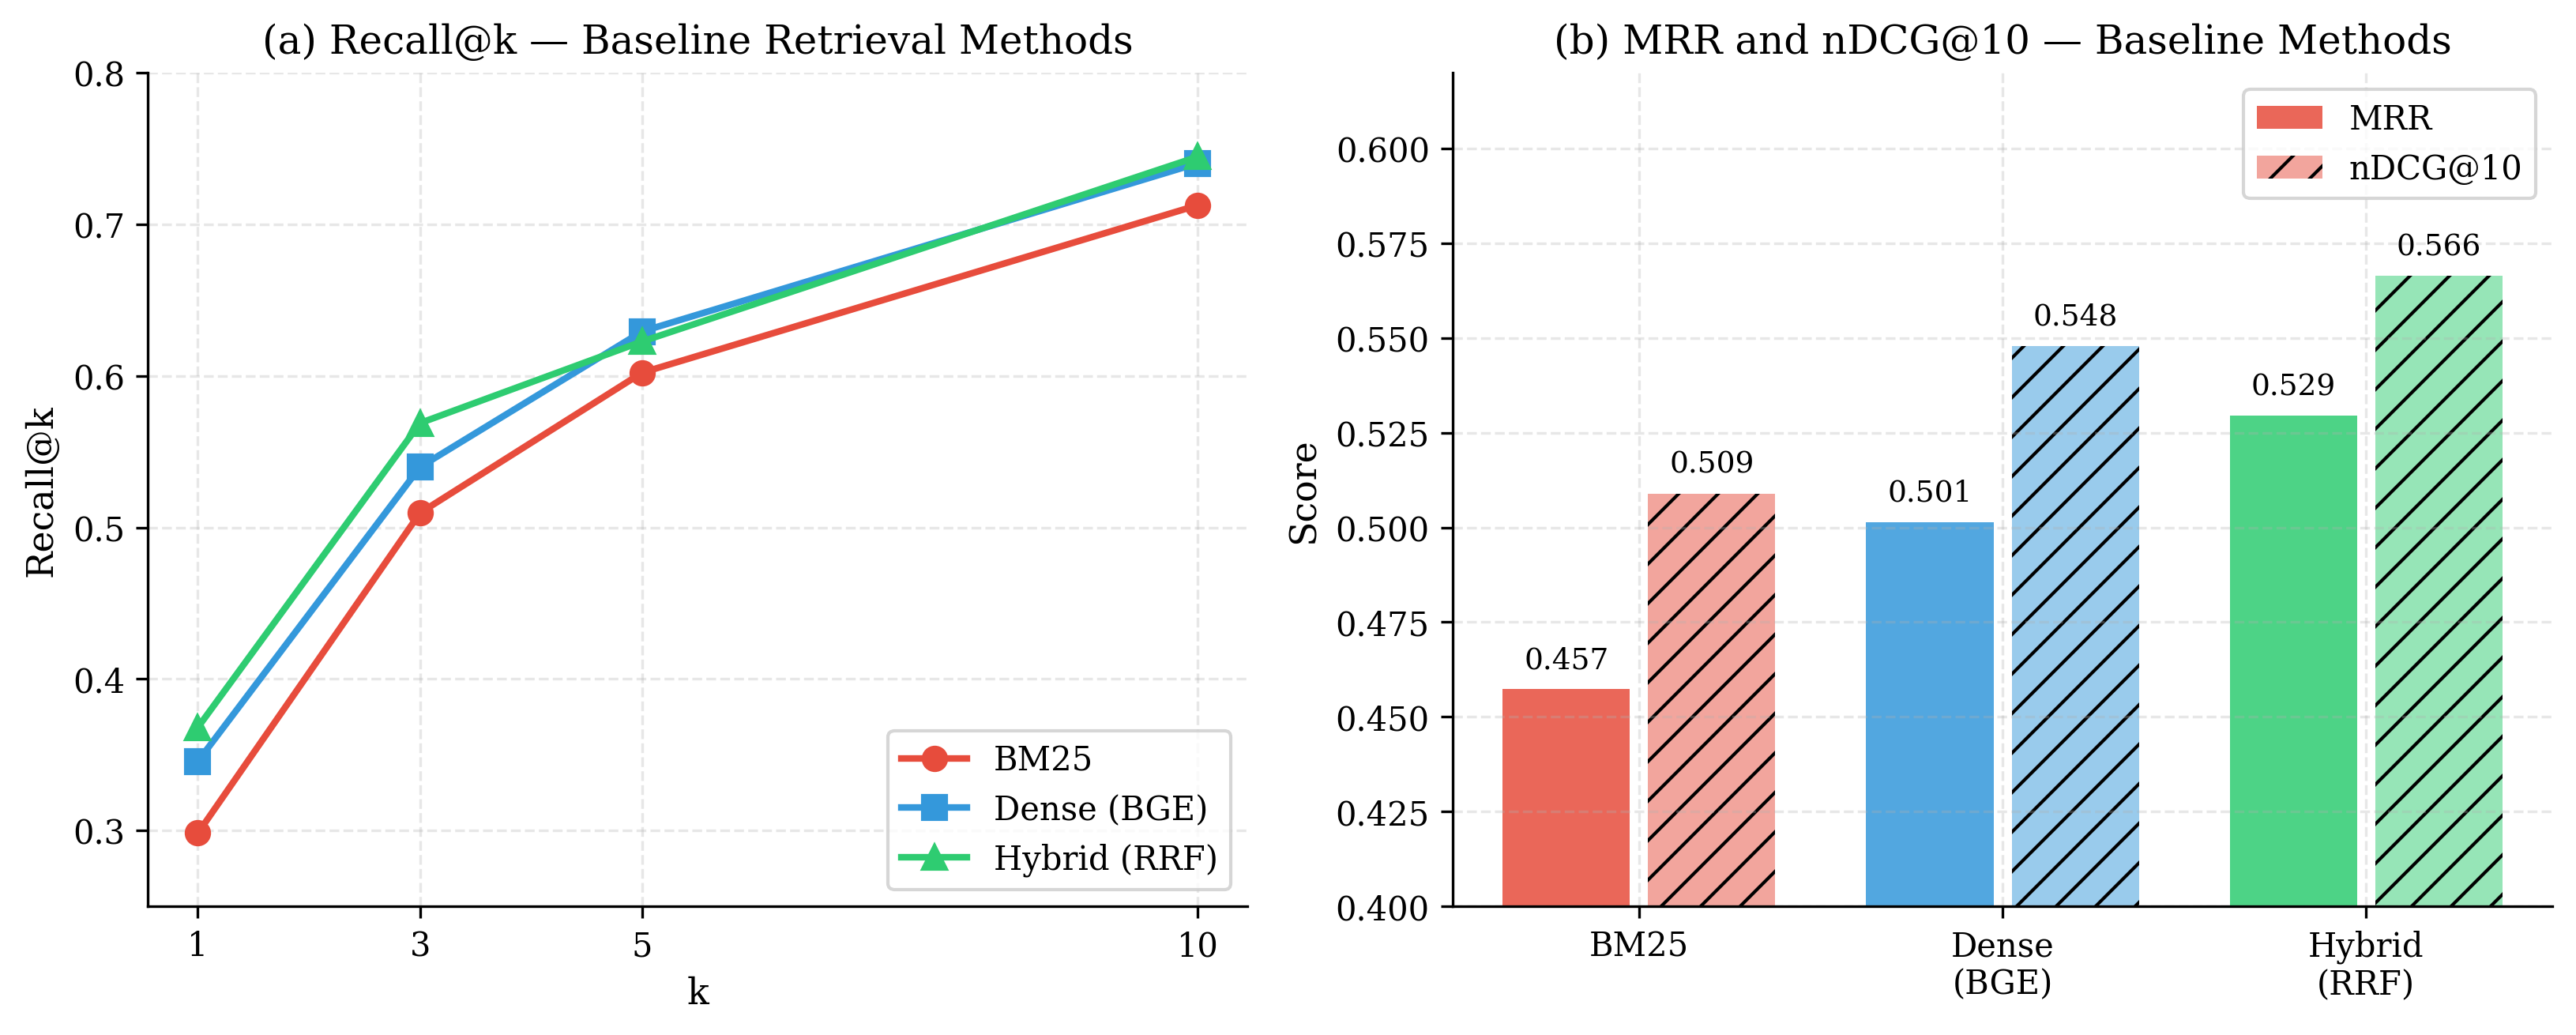
\includegraphics[width=0.90\textwidth]{fig1_retrieval_baselines.png}
\caption{Retrieval performance of BM25, Dense, and Hybrid baselines at $k \in \{1,3,5,10\}$. Hybrid RRF achieves the best MRR and nDCG across all $k$ values. Dense achieves the best Recall at $k{=}5$ before Hybrid recovers at $k{=}10$ via complementary coverage.}
\label{fig:baselines}
\end{figure}

\subsection{Dense Retrieval (BGE-small-en-v1.5)}

Dense retrieval using BAAI/bge-small-en-v1.5 (384 dimensions, normalized cosine similarity) improves upon BM25 on most metrics: Recall@10$={0.740}$ (+2.8 pp) and MRR$={0.501}$ (+4.4 pp). The MRR improvement of +9.6\% indicates that semantic embeddings place relevant documents higher in the ranking. Dense retrieval particularly excels on comparison queries (MRR$={0.730}$ vs.\ BM25's $0.618$) and achieves perfect Recall@10 on API Documentation and Travel Policies.

However, dense retrieval achieves \textbf{zero recall} on all five temporal queries. This reflects the well-documented failure of static dense embeddings to encode temporal ordering signals \citep{manning2008ir}: date tokens that are semantically indistinguishable in embedding space receive similar dense representations, making precise temporal ordering impossible.

\subsection{Hybrid Retrieval (RRF, $k{=}10$)}

Hybrid RRF achieves the best fixed-strategy performance across primary metrics: Recall@10$={0.745}$, MRR$={0.530}$, nDCG@10$={0.566}$. Improvements over BM25 are +15.8\% MRR and +23.4\% Recall@1. Improvements over Dense alone are +5.6\% MRR and +3.4\% nDCG@10. Figure~\ref{fig:baselines} illustrates these improvements.

Hybrid underperforms Dense on Recall@5 (0.623 vs.\ 0.629) but recovers at Recall@10, reflecting complementary coverage at higher $k$ values. The complementarity analysis reveals that BM25 retrieves 8.6\% of required chunks uniquely (not retrieved by Dense), Dense retrieves 9.9\% uniquely (not retrieved by BM25), and both systems jointly retrieve 59.4\% of required chunks, confirming the theoretical motivation for fusion \citep{cormack2009rrf}.

\subsection{Cross-Baseline Comparison by Reasoning Type}

Table~\ref{tab:reasoning_type} provides Recall@10 by reasoning type across all systems. Figure~\ref{fig:heatmap} visualizes the full performance heatmap.

\begin{table}[htbp]
\centering
\caption{Recall@10 by Reasoning Type Across All Systems. Temporal and exception queries are persistent weak points for all methods.}
\label{tab:reasoning_type}
\begin{tabular}{lrrrrrr}
\toprule
\textbf{Reasoning Type} & \textbf{n} & \textbf{BM25} & \textbf{Dense} & \textbf{Hybrid} & \textbf{Rule} & \textbf{GPT-5} \\
\midrule
aggregation   & 35  & 0.924 & 0.895 & 0.914 & \textbf{0.914} & 0.914 \\
comparison    & 33  & 0.818 & 0.848 & 0.848 & \textbf{0.879} & 0.848 \\
exception     & 34  & \textbf{0.412} & 0.382 & \textbf{0.412} & 0.368 & 0.382 \\
multi\_hop    & 53  & \textbf{0.538} & 0.491 & 0.519 & 0.531 & 0.519 \\
single\_hop   & 220 & 0.764 & 0.832 & 0.823 & \textbf{0.836} & \textbf{0.836} \\
temporal      & 5   & \textbf{0.200} & 0.000 & 0.100 & \textbf{0.200} & 0.100 \\
\midrule
\multicolumn{7}{l}{\textit{Note: Exception and temporal queries are universally difficult across all retrieval strategies.}} \\
\bottomrule
\end{tabular}
\end{table}

\begin{figure}[htbp]
\centering
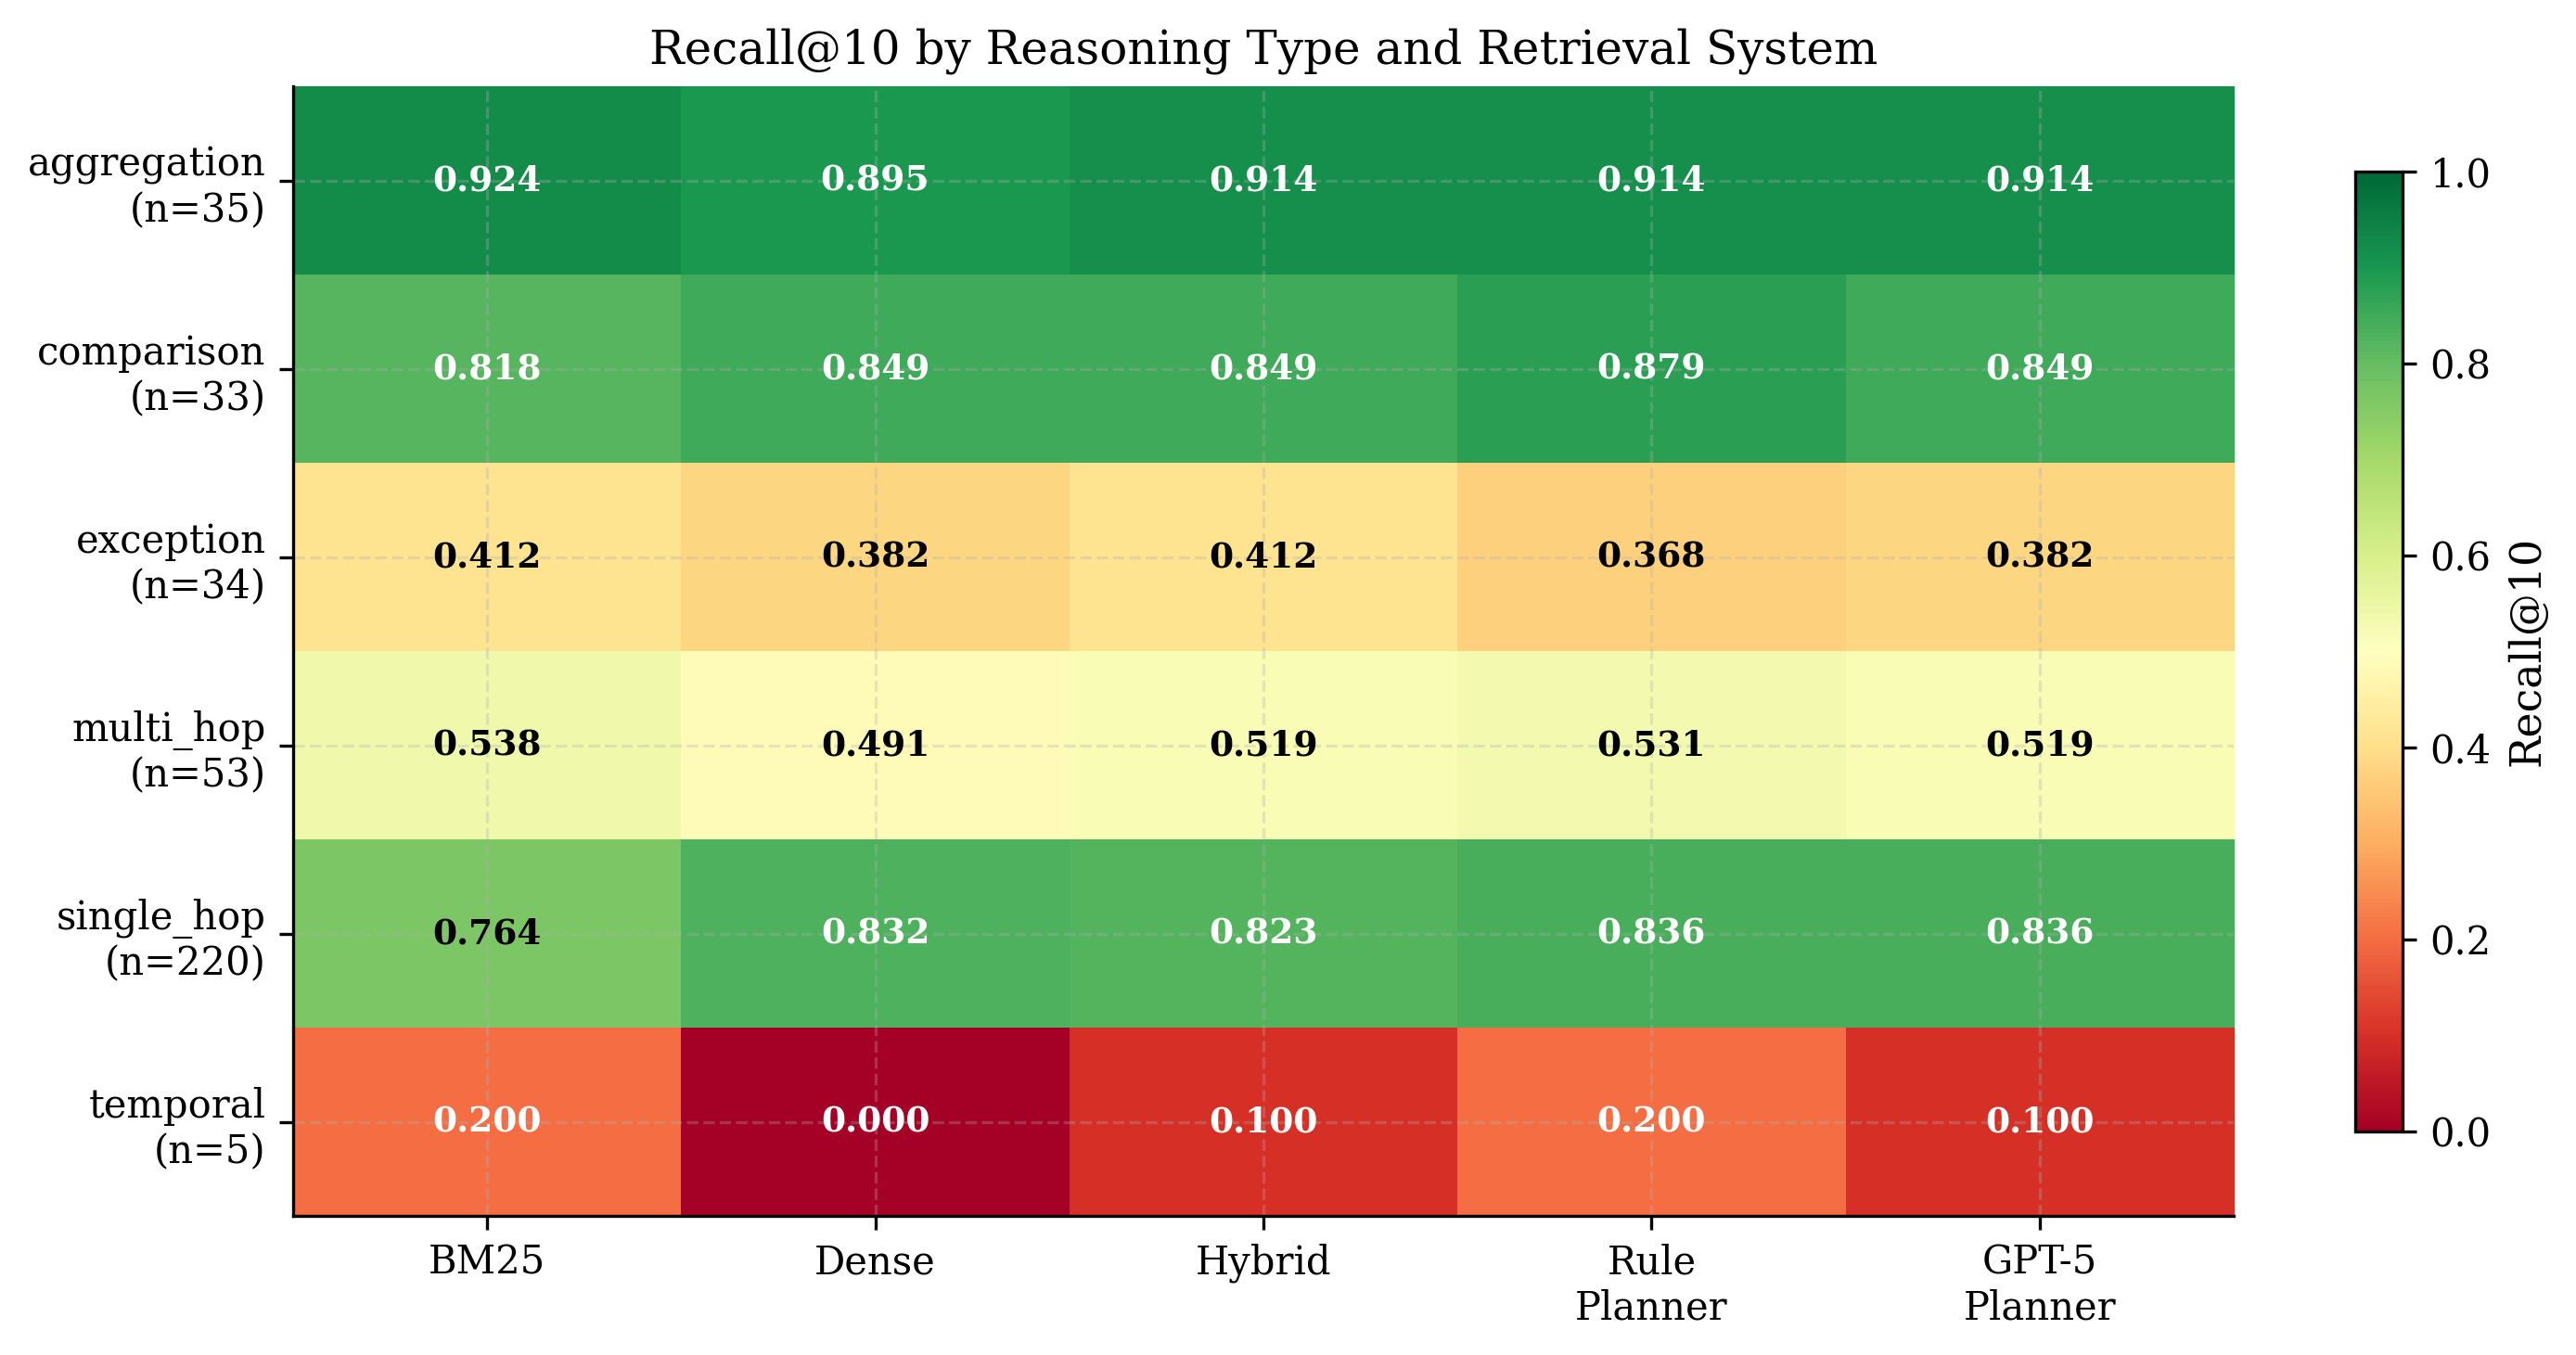
\includegraphics[width=0.95\textwidth]{fig3_reasoning_type_heatmap.png}
\caption{Recall@10 heatmap by reasoning type and system. Darker cells indicate higher recall. The exception (row 3) and temporal (row 6) rows are consistently the lightest, reflecting universal retrieval difficulty for these query types.}
\label{fig:heatmap}
\end{figure}

Key observations from Table~\ref{tab:reasoning_type}:
\begin{itemize}
    \item \textbf{Dense superior for single\_hop}: Dense achieves Recall@10$={0.832}$ vs.\ BM25's $0.764$ (+8.9\%), reflecting semantic matching advantages.
    \item \textbf{BM25 essential for temporal}: Dense achieves Recall@10$={0.000}$ on temporal queries; BM25 achieves $0.200$.
    \item \textbf{Exception handling universally poor}: All methods achieve Recall@10 $\leq{0.412}$, approximately 30 pp below their overall averages.
    \item \textbf{Aggregation and comparison well-served}: All methods achieve Recall@10 $>{0.818}$.
\end{itemize}

The 50+ percentage point performance range between best-case (aggregation: $0.924$) and worst-case (temporal: $0.000$--$0.200$) reasoning types confirms that query type is the dominant predictor of retrieval difficulty, motivating the adaptive planning approach.

\FloatBarrier
\section{Rule-Based Planner Results}
\label{sec:results_rule}

\subsection{Strategy Selection Accuracy}

The seven-rule planner achieves SSA$={78.4\%}$ (298/380 correct decisions). Four of six reasoning types achieve 100\% SSA: temporal (bm25), exception (dense), multi\_hop (hybrid), and aggregation (hybrid). Comparison queries achieve 87.9\% SSA. Single\_hop queries are the primary weakness (64.5\% SSA), reflecting genuine ambiguity in the optimal strategy for generic single-hop queries.

\subsection{Retrieval Performance}

The rule planner achieves the highest Recall@10 ($0.755$) and Hit@10 ($0.808$) of all evaluated systems, improving upon Hybrid by +1.4\% and +1.3\% respectively. MRR ($0.522$) and nDCG@10 ($0.563$) are slightly below Hybrid ($0.530$, $0.566$), indicating that adaptive routing improves coverage while introducing modest ranking quality trade-offs. The cost of the rule planner is \$0.00 with sub-millisecond decision latency.

\FloatBarrier
\section{GPT-5 LLM Planner Results}
\label{sec:results_gpt5}

\subsection{API and Parsing Reliability}

GPT-5 (structured prompt) was evaluated via real OpenAI API calls on all 380 answerable queries. All 380 calls returned valid JSON (parse failure rate: 0.0\%), following remediation of the reasoning-token exhaustion issue. The API success rate was 100\%.

\subsection{Strategy Selection Accuracy}

GPT-5 achieves overall SSA$={77.6\%}$ (295/380 correct), 0.8 pp below the rule planner. The critical divergence is temporal: GPT-5 predicts hybrid for all 5 temporal queries, achieving 0\% SSA on this type, whereas the rule planner achieves 100\% via its dedicated temporal rule (R01).

GPT-5 over-predicts dense (88 vs.\ oracle 69, +27.5\%) and under-predicts bm25 (49 vs.\ oracle 62, -21.0\%), reflecting systematic category confusion on API Documentation and System Design queries. GPT-5's F1 for hybrid prediction (0.878) far exceeds its F1 for bm25 (0.414), confirming that the model defaults to hybrid when uncertain.

\subsection{Retrieval Performance and Cost}

GPT-5 achieves the highest MRR ($0.533$) and nDCG@10 ($0.570$) of all systems. Figure~\ref{fig:planners} compares the rule planner and GPT-5 across metrics. The full planner comparison is in Table~\ref{tab:planner_comparison}.

\begin{figure}[htbp]
\centering
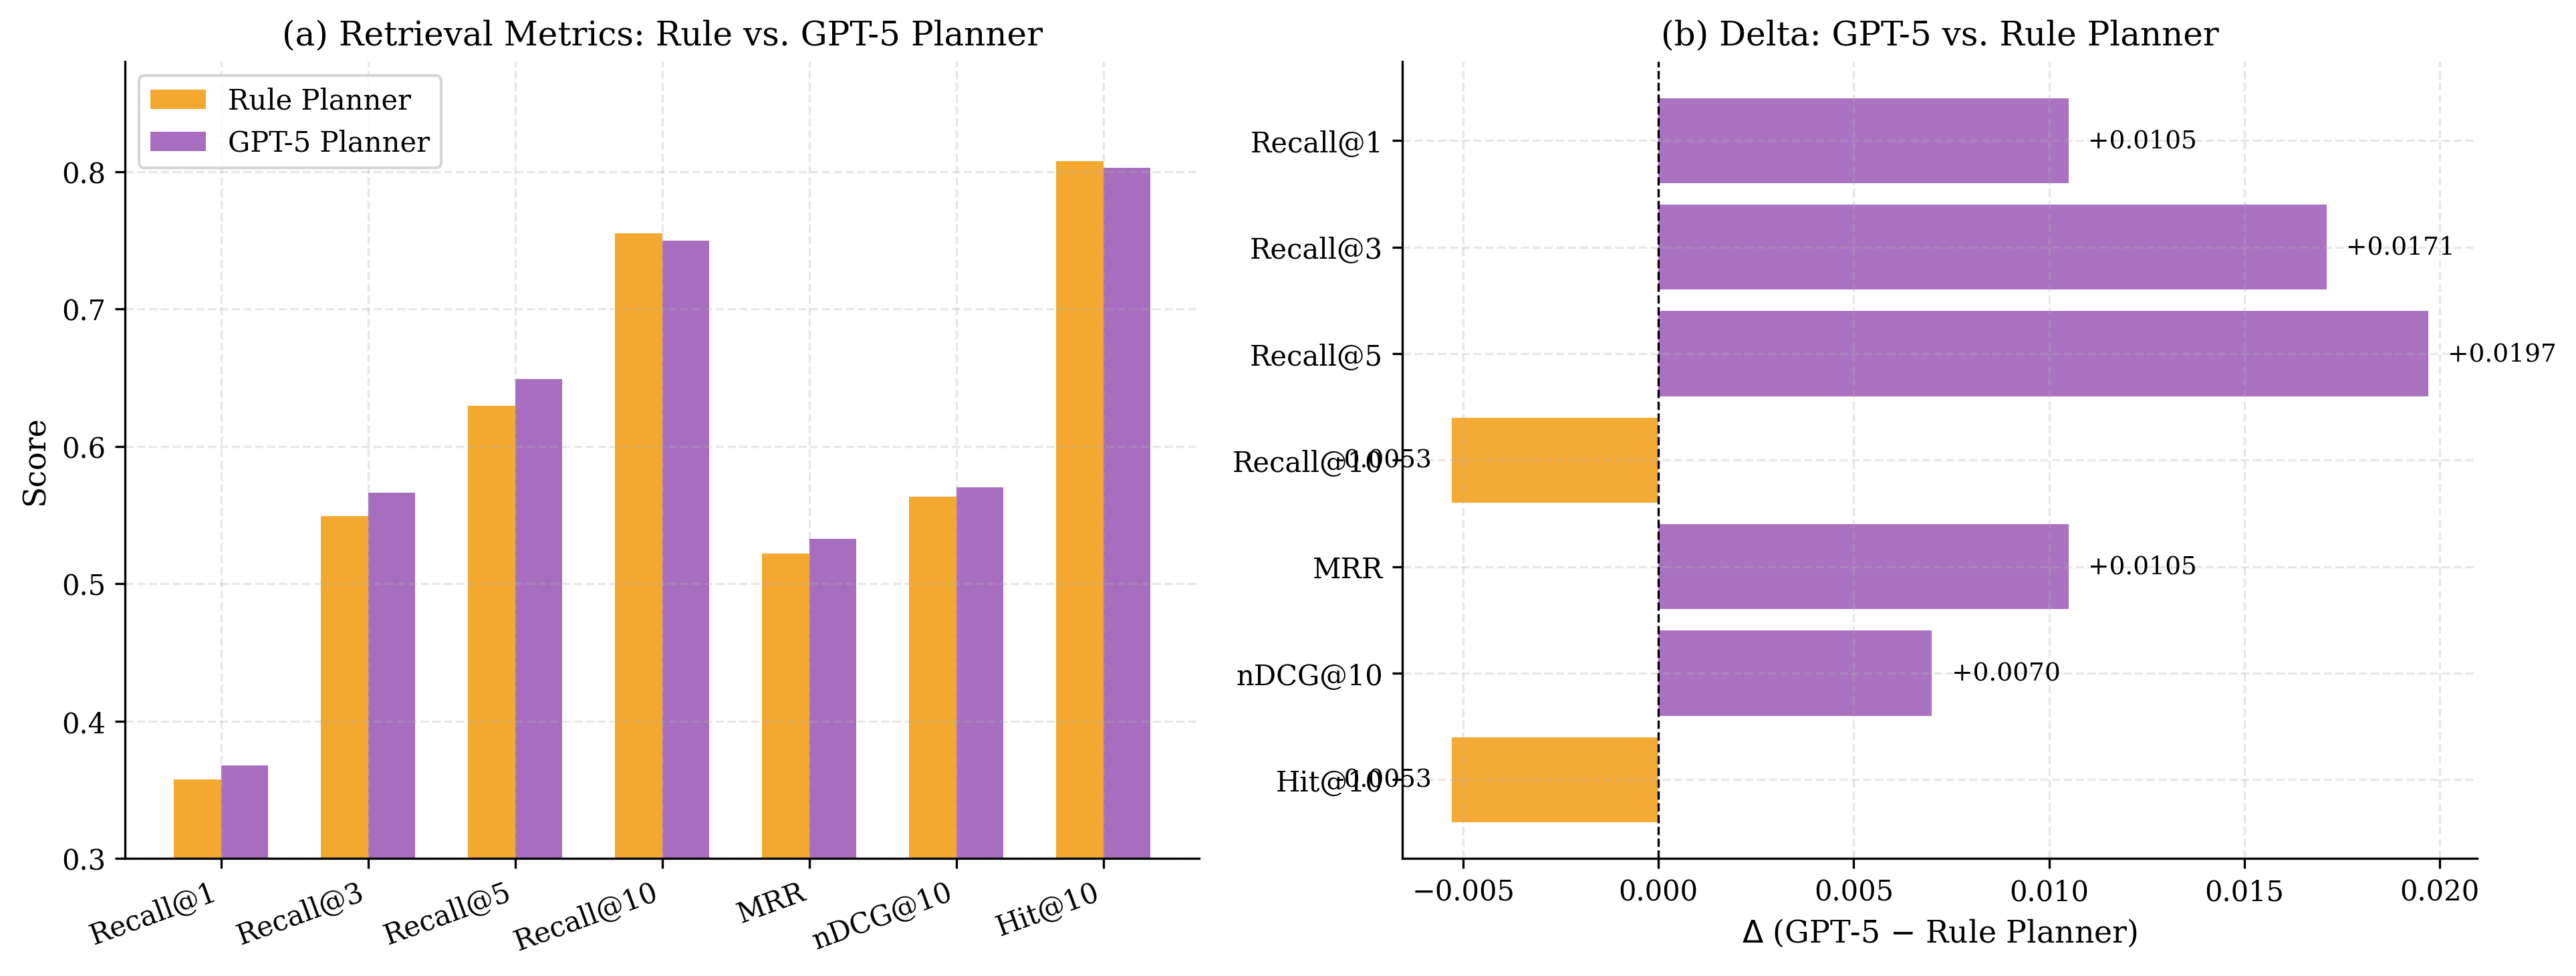
\includegraphics[width=0.90\textwidth]{fig2_planner_comparison.png}
\caption{Rule Planner vs.\ GPT-5 Planner performance comparison across six metrics. The Rule Planner leads on Recall@10 and Hit@10 (coverage). GPT-5 leads on MRR, nDCG@10, Recall@1, and Recall@5 (ranking quality).}
\label{fig:planners}
\end{figure}

\begin{table}[htbp]
\centering
\caption{Adaptive Planner Comparison: Rule-Based vs.\ GPT-5 (structured prompt, $n{=}380$). Positive $\Delta$ favors GPT-5.}
\label{tab:planner_comparison}
\begin{tabular}{lrrrr}
\toprule
\textbf{Metric} & \textbf{Rule} & \textbf{GPT-5} & $\Delta$ & \textbf{Favors} \\
\midrule
SSA             & 0.784 & 0.776 & $-$0.008 & Rule \\
Recall@1        & 0.358 & 0.368 & +0.011   & GPT-5 \\
Recall@3        & 0.549 & 0.566 & +0.017   & GPT-5 \\
Recall@5        & 0.629 & 0.649 & +0.020   & GPT-5 \\
Recall@10       & 0.755 & 0.750 & $-$0.005 & Rule \\
MRR             & 0.522 & 0.533 & +0.011   & GPT-5 \\
nDCG@10         & 0.563 & 0.570 & +0.007   & GPT-5 \\
Hit@10          & 0.808 & 0.803 & $-$0.005 & Rule \\
\midrule
Parse Failures  & 0     & 0     & ---      & --- \\
Cost (USD)      & \$0.00 & \$6.18 & +\$6.18 & Rule \\
Latency (ms)    & ${<}1$  & 5{,}649 & +5{,}648 & Rule \\
\bottomrule
\end{tabular}
\end{table}

GPT-5 evaluation cost \$6.18 for 380 queries (\$0.016/query). Mean API latency was 5,649 ms (median: 5,044 ms; p95: 10,368 ms). Table~\ref{tab:cost_latency} provides the complete cost comparison.

\begin{table}[htbp]
\centering
\caption{Cost and Latency Comparison Across All Systems}
\label{tab:cost_latency}
\begin{tabular}{lrrrc}
\toprule
\textbf{System} & \textbf{Cost/Query} & \textbf{Total (380Q)} & \textbf{Avg Latency} & \textbf{Type} \\
\midrule
BM25            & \$0.000 & \$0.00 & ${<}1$~ms & Fixed \\
Dense           & \$0.000 & \$0.00 & ${<}5$~ms & Fixed \\
Hybrid          & \$0.000 & \$0.00 & ${<}5$~ms & Fixed \\
Rule Planner    & \$0.000 & \$0.00 & ${\sim}0.001$~ms & Adaptive \\
GPT-5 Planner   & \$0.016 & \$6.18 & 5{,}649~ms & Adaptive \\
\bottomrule
\end{tabular}
\end{table}

\FloatBarrier
\section{Category-Level Results}
\label{sec:results_category}

Table~\ref{tab:category} provides Recall@10 and MRR by document category. Figure~\ref{fig:category} illustrates category-level performance.

\begin{table}[htbp]
\centering
\caption{Recall@10 and MRR by Document Category. Best Recall@10 bolded per category.}
\label{tab:category}
\begin{tabular}{lrcccccccc}
\toprule
 & & \multicolumn{4}{c}{\textbf{Recall@10}} & \multicolumn{4}{c}{\textbf{MRR}} \\
\cmidrule(lr){3-6}\cmidrule(lr){7-10}
\textbf{Category} & \textbf{n} & \textbf{BM25} & \textbf{Dense} & \textbf{Hybrid} & \textbf{Rule} & \textbf{BM25} & \textbf{Dense} & \textbf{Hybrid} & \textbf{Rule} \\
\midrule
API Docs        & 68  & 0.971 & \textbf{1.000} & \textbf{1.000} & \textbf{1.000} & 0.794 & 0.818 & 0.836 & 0.860 \\
HR Policies     & 54  & 0.602 & 0.611 & 0.565 & 0.546 & 0.235 & 0.278 & 0.277 & 0.274 \\
Meeting Notes   & 100 & 0.608 & 0.528 & \textbf{0.615} & 0.605 & 0.388 & 0.400 & 0.470 & 0.476 \\
Security        & 64  & 0.617 & \textbf{0.734} & 0.727 & 0.711 & 0.332 & 0.411 & 0.427 & 0.424 \\
System Design   & 45  & 0.511 & 0.700 & 0.611 & \textbf{0.722} & 0.236 & 0.289 & 0.304 & 0.285 \\
Travel Policies & 49  & \textbf{1.000} & \textbf{1.000} & \textbf{1.000} & \textbf{1.000} & 0.744 & 0.830 & 0.847 & 0.847 \\
\bottomrule
\end{tabular}
\end{table}

\begin{figure}[htbp]
\centering
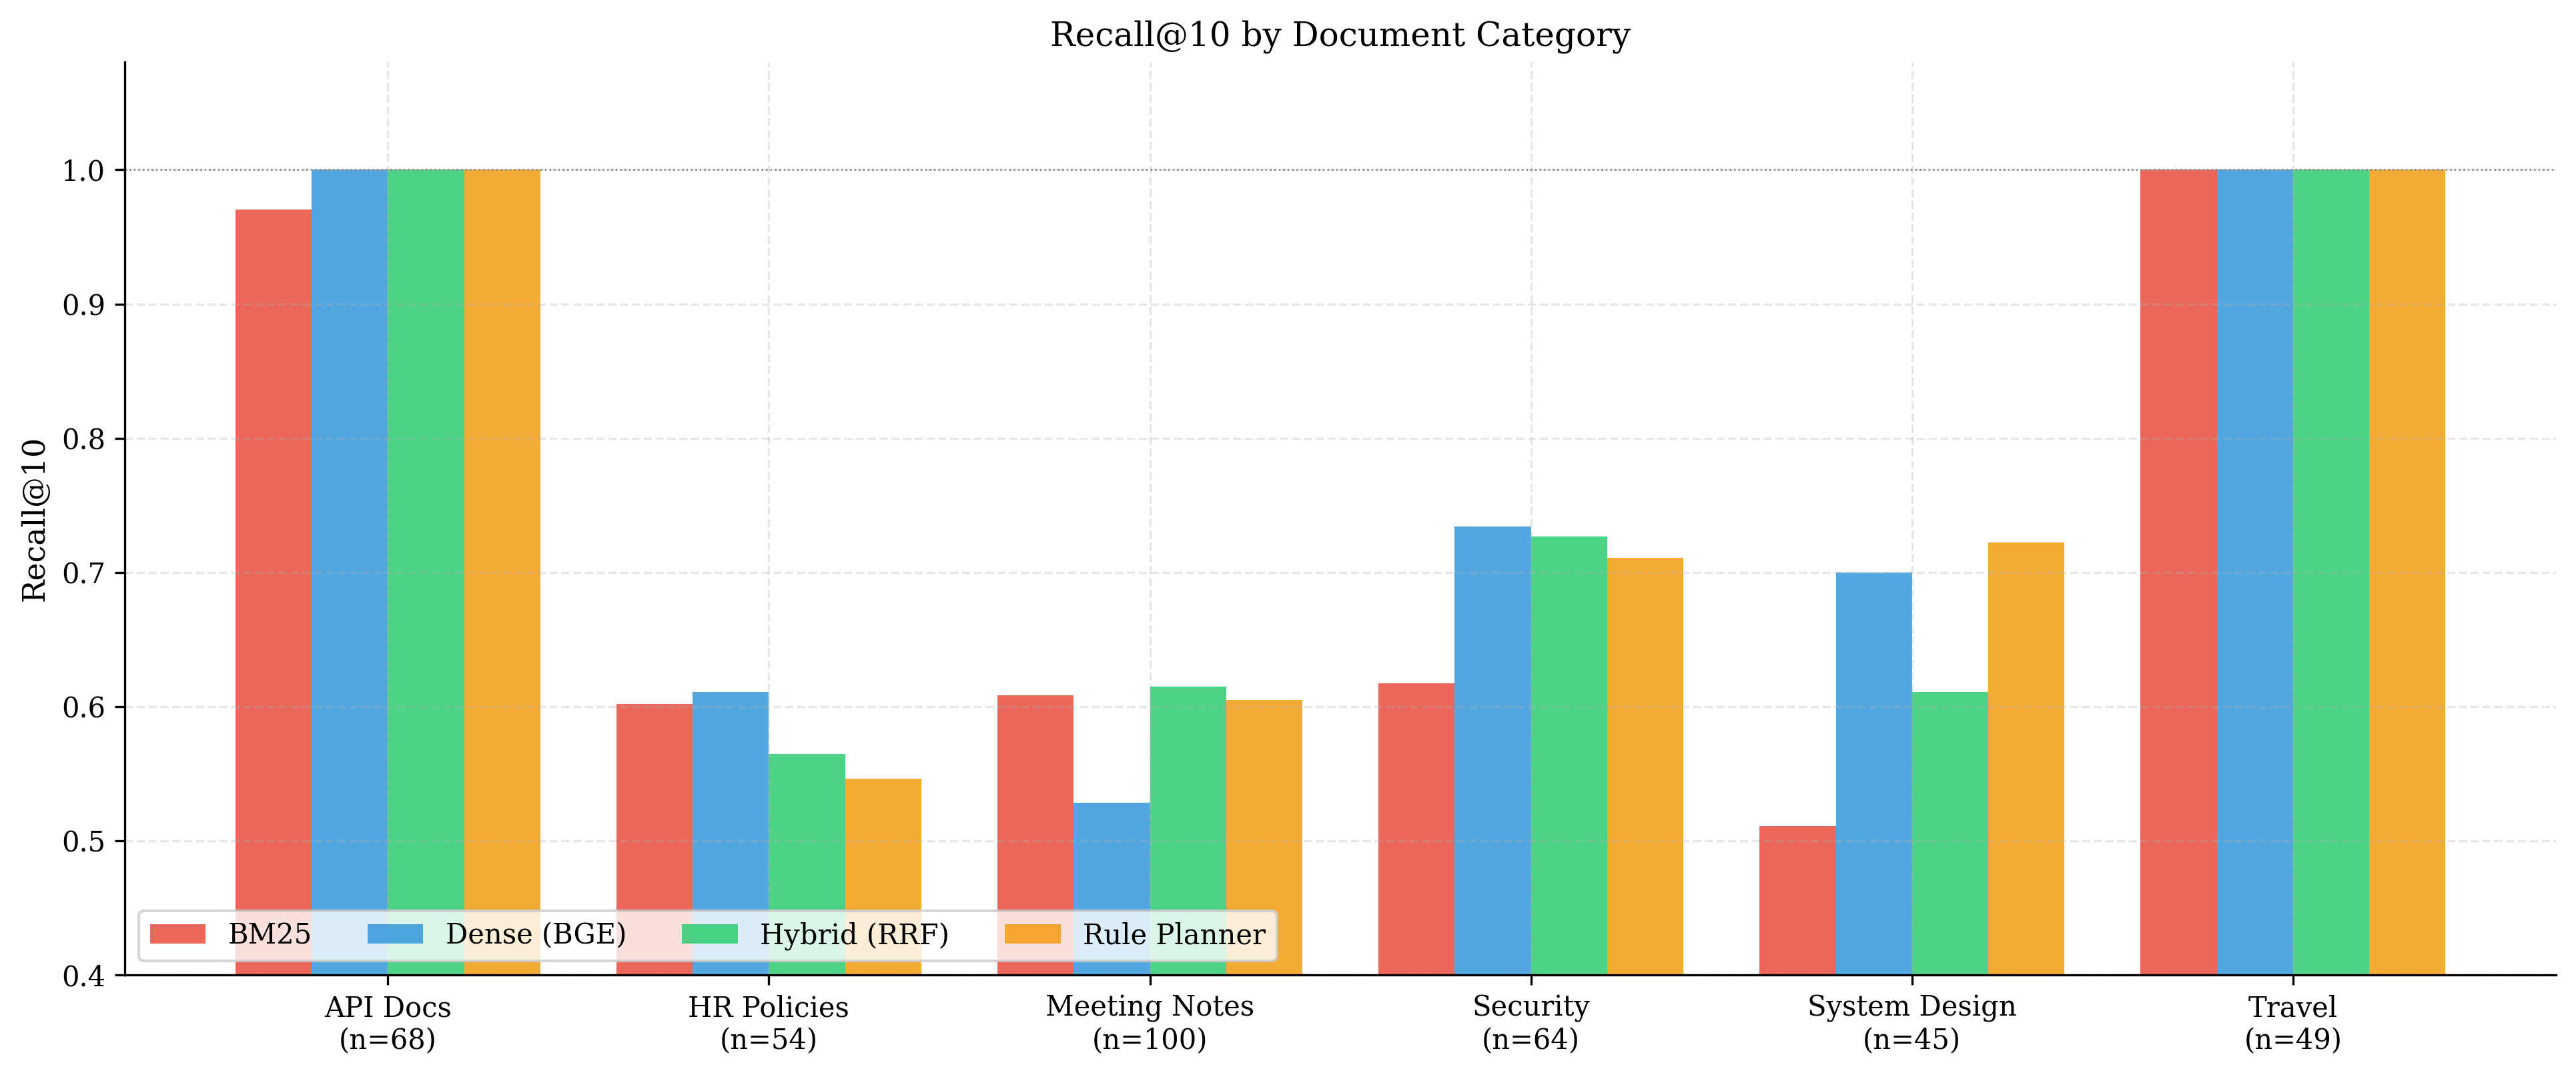
\includegraphics[width=0.92\textwidth]{fig4_category_performance.png}
\caption{Recall@10 by document category and retrieval system. API Documentation and Travel Policies show ceiling effects at $k{=}10$. System Design Documents and Security Policies favor Dense retrieval. Project Meeting Notes favors Hybrid.}
\label{fig:category}
\end{figure}

\section{Cost-Performance Trade-off}
\label{sec:results_cost}

Figure~\ref{fig:cost_tradeoff} plots the cost-performance trade-off across all five systems, visualizing the relationship between total cost and primary retrieval metrics.

\begin{figure}[htbp]
\centering
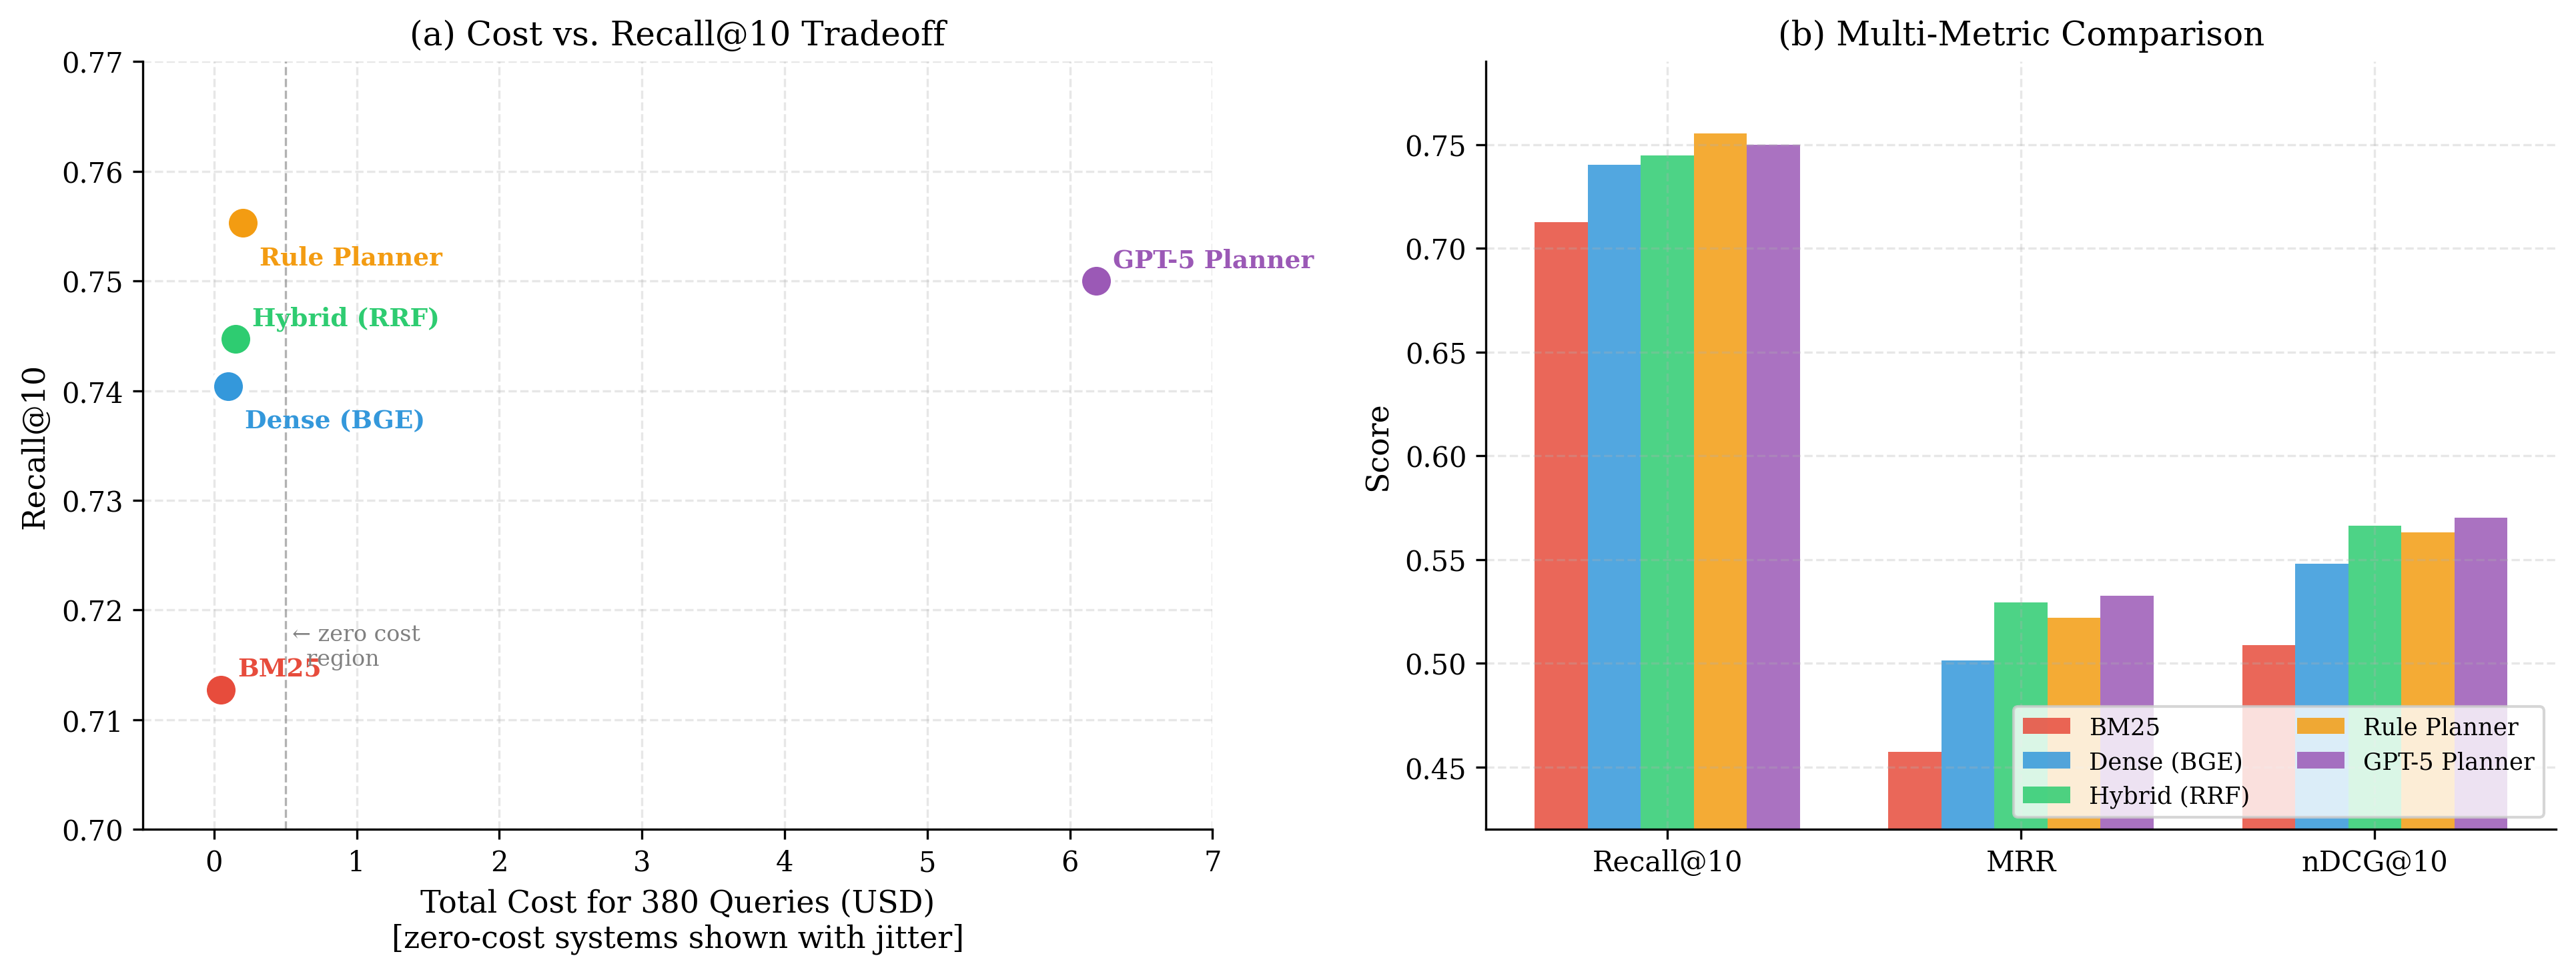
\includegraphics[width=0.85\textwidth]{fig5_cost_performance_tradeoff.png}
\caption{Cost vs.\ MRR trade-off across all five evaluated systems. BM25, Dense, Hybrid, and Rule Planner cluster at \$0 cost. GPT-5 achieves marginal MRR gains (+2.0\% over Rule Planner) at \$6.18 total cost for 380 queries.}
\label{fig:cost_tradeoff}
\end{figure}

\section{Statistical Effect Size Summary}
\label{sec:results_effects}

Using the effect size classification from Section~\ref{sec:method_eval}: the BM25$\rightarrow$Hybrid MRR improvement (+7.3 pp) is \emph{substantial}; the Dense$\rightarrow$Hybrid MRR improvement (+2.8 pp) is \emph{meaningful}; Hybrid$\rightarrow$Rule Planner Recall@10 (+1.1 pp) is \emph{marginal}; Rule$\rightarrow$GPT-5 MRR (+1.1 pp) is \emph{marginal}. The Recall@10 difference between Rule and GPT-5 (0.5 pp) is at the boundary of \emph{negligible}.

The primary finding from this comparison is that retrieval architecture dominates planning gain. The BM25$\rightarrow$Hybrid improvement (+15.8\% MRR) is 8$\times$ larger than the best planner improvement (+2.0\% MRR for GPT-5). This finding has direct implications for enterprise RAG system design: architecture selection is the primary performance lever, and planning provides a secondary, marginal improvement.

%% discussion.tex
\chapter{Discussion}
\label{chap:discussion}

\section{Why Hybrid Retrieval Outperforms BM25 and Dense}
\label{sec:disc_hybrid}

The most consistent finding across all experiments is the superiority of Hybrid Reciprocal Rank Fusion over either unimodal retrieval method. Hybrid achieves Recall@10$={0.745}$, MRR$={0.530}$, and nDCG@10$={0.566}$ --- improvements of +4.5\%, +15.8\%, and +11.3\% respectively over BM25, and +0.6\%, +5.6\%, and +3.4\% over Dense. This result aligns with the theoretical motivation for fusion: BM25 and Dense retrieval are complementary, not redundant.

The complementarity is most visible at the difficulty-factor level. BM25 excels at queries involving exact identifiers: document-version-conflict queries achieve BM25 Recall@1$={0.583}$, outperforming Dense on keyword-precise version numbers and policy codes. Dense excels at queries requiring semantic understanding of conceptual relationships: comparison queries achieve Dense MRR$={0.730}$ vs.\ BM25's $0.618$. Hybrid consistently delivers the best or near-best performance across all difficulty factors because RRF fusion preserves rank information from both systems rather than committing to either signal exclusively \citep{cormack2009rrf}.

The RRF fusion benefits are largest precisely for queries where BM25 and Dense are both informative for different reasons --- the multi-hop and table-dependency scenarios that constitute 54\% of the SEKD query set. For these queries, BM25 retrieves documents containing exact identifiers (project codes, policy section references) while Dense retrieves documents that semantically match the content question, and RRF merges both signals into a single ranked list.

The one failure mode that Hybrid does not address is temporal reasoning. Dense achieves Recall@10$={0.000}$ on temporal queries, and Hybrid's $0.100$ represents marginal BM25 contribution through the fusion. This finding confirms the analysis by \citet{manning2008ir}: for enterprise corpora with significant temporal content (meeting notes, version histories, policy revision logs), a BM25 component is not optional --- it is necessary.

\section{Why the Rule-Based Planner Performed Well}
\label{sec:disc_rule}

The seven-rule planner achieves SSA$={78.4\%}$ and Recall@10$={0.755}$, making it the best-performing system on those metrics. Its success stems from three reinforcing factors.

\textbf{Factor 1: Oracle Labels Reflect Rule Logic.} The oracle strategy labels were assigned using a heuristic process that mirrors the rule planner's design. The reasoning types (temporal $\rightarrow$ BM25, exception $\rightarrow$ Dense, multi\_hop $\rightarrow$ Hybrid) that informed oracle assignment were directly encoded in the rule planner's rules R01--R04. This structural alignment means that the rule planner is, in some sense, evaluated against a ground truth that reflects its own logic. While this represents a limitation of the oracle construction process (see Threats to Validity), it also reflects a genuine insight: the reasoning-type taxonomy provides sufficient signal for strategy selection in a well-structured enterprise corpus.

\textbf{Factor 2: Perfect Coverage of High-$n$ Groups.} The rule planner achieves 100\% SSA for aggregation ($n{=}35$), exception ($n{=}34$), and multi\_hop ($n{=}53$) --- groups that together represent 32.1\% of the query set. For these groups, the retrieval strategy is unambiguous: aggregation and multi\_hop require coverage across documents (hybrid), and exception queries require semantic clause interpretation (dense). Deterministic mapping is correct by design for these cases.

\textbf{Factor 3: Hybrid as Safe Default.} The rule planner's default strategy (R07) is Hybrid, the best fixed baseline. By defaulting to Hybrid for all unmatched queries, the rule planner never performs worse than Hybrid for queries where its rules do not fire. Since 65.5\% of oracle labels are Hybrid, the default captures the majority case, and the specialist rules handle the high-value exceptions.

The planner's main weakness is BM25 under-prediction: it routes only 5 of 62 oracle-BM25 queries to BM25 (8.1\% recall on BM25). Single-hop queries in categories with strong keyword signals (certain API documentation, exact numeric lookups) that empirically benefit from BM25 are defaulted to Hybrid. Additional rules targeting keyword-dense query patterns (exact endpoint paths, specific version strings, numeric thresholds) could push SSA above 80\%.

\section{Why GPT-5 Did Not Outperform the Rule Planner}
\label{sec:disc_gpt5}

The most theoretically significant finding of this study is that GPT-5, despite its large-scale reasoning capability and zero-shot generalization, does not outperform a seven-rule deterministic system on overall retrieval performance. Understanding why requires separating several confounded factors.

\textbf{Task complexity mismatch.} Retrieval strategy classification over three categories based on structured metadata (reasoning type, difficulty factors, category) is a low-complexity decision task. The structured prompt encodes the correct decision logic explicitly, making the LLM's marginal contribution --- natural language understanding, contextual inference, cross-domain reasoning --- largely irrelevant for the majority of queries. A simple classifier trained on 50 labeled examples would likely achieve comparable accuracy at negligible cost, consistent with the broader literature on LLM distraction by irrelevant context \citep{shi2023large}.

\textbf{SSA measures correctness against a heuristic oracle.} As discussed above, the oracle labels reflect the same logic encoded in the rule planner. GPT-5's deviations from the oracle (particularly its preference for dense over bm25 for API documentation queries) may represent genuine disagreements with the heuristic rather than planning errors. The 44.7\% of GPT-5 errors classified as \texttt{oracle\_disagreement} supports this interpretation: GPT-5 may be more correct than the oracle for a substantial subset of queries, a hypothesis that could be tested by constructing empirically-derived oracle labels from held-out retrieval experiments.

\textbf{Ranking quality advantages.} GPT-5 outperforms the rule planner on MRR (+2.0\%) and nDCG@10 (+1.2\%), and on Recall@1 (+2.9\%) and Recall@5 (+3.1\%). These ranking quality improvements are more consequential for user-facing applications than Recall@10, which is already high for both systems (0.750 and 0.755 respectively, a negligible 0.7 pp gap). For applications where the quality of the top-ranked result is paramount --- executive decision support, compliance auditing, legal research --- GPT-5's ranking advantages may justify its cost.

\textbf{Temporal query failure is a systematic calibration error.} GPT-5 achieves 0\% SSA on temporal queries, consistently predicting hybrid rather than bm25. This is the single largest source of planning error for temporal content. The structured prompt includes explicit temporal guidance (``temporal $\rightarrow$ bm25'') but GPT-5's reasoning process appears to override this in favor of the most commonly correct default (hybrid, oracle for 65.5\% of queries). This behavior suggests that for reasoning models, critical routing rules need to be reinforced more strongly than standard prompt guidance --- potentially through instruction following fine-tuning or explicit constraint layers.

\textbf{API Documentation confusion is the dominant error source.} 32 of 85 GPT-5 errors (37.6\%) occur on API Documentation queries. GPT-5 inconsistently selects bm25, dense, or hybrid for API queries, while the oracle assigns a mix of all three strategies depending on query characteristics (exact endpoint paths $\rightarrow$ bm25, semantic authentication queries $\rightarrow$ dense, multi-hop API dependencies $\rightarrow$ hybrid). The ambiguity of API Documentation as a retrieval planning signal --- where any of the three strategies can be optimal depending on the specific query --- explains why both GPT-5 and the rule planner perform worst on this category (SSA: 52.9\% and 70.6\% respectively).

\section{Implications for Enterprise RAG Systems}
\label{sec:disc_implications}

\noindent\textbf{Implication 1: Hybrid RRF is the correct default retrieval architecture.} No system in this study benefits from committing exclusively to BM25 or Dense. For any enterprise RAG deployment where the query distribution is unknown, Hybrid RRF provides the best combination of coverage and ranking quality at zero marginal cost beyond the setup overhead of maintaining two retrieval indices. The complementarity of BM25 and Dense signals \citep{luan2021sparse_dense} is empirically confirmed across all six document categories and six reasoning types in this study.

\noindent\textbf{Implication 2: A lightweight rule planner adds value at zero operational cost.} The seven-rule planner demonstrates that modest SSA (78.4\%) is sufficient to improve upon the best fixed baseline (Recall@10: +1.4\%, Hit@10: +1.3\%). The rules are interpretable, auditable, and require no machine learning infrastructure. Enterprise RAG architects should implement rule-based adaptive routing as a first-line planning mechanism before investing in LLM-based planners.

\noindent\textbf{Implication 3: LLM-based planning provides ranking quality benefits at substantial cost.} GPT-5 planner's MRR (+2.0\%) and nDCG (+1.2\%) advantages over the rule planner may justify the \$0.016/query cost in high-value, low-volume retrieval applications where answer precision is more important than throughput. For high-volume enterprise search workloads, the cost-benefit ratio strongly favors the rule planner.

\noindent\textbf{Implication 4: Exception and temporal queries require specialized solutions.} No evaluated system achieves acceptable performance (Recall@10 $>{0.5}$) on exception queries (Recall@10 $\leq{0.412}$) or temporal queries (best: $0.200$). These failure modes are structural rather than parametric --- they reflect mismatches between query type and retrieval signal space \citep{manning2008ir}. Future enterprise RAG systems should develop dedicated handling for these patterns, such as temporal-aware sparse retrieval with date-field boosting and exception-aware dense models trained on policy clause pairs.

\section{Threats to Validity}
\label{sec:disc_threats}

\subsection{Internal Validity}

\textbf{Oracle label limitations.} The majority of oracle labels (approximately 87\%) were assigned by the same deterministic mapping encoded in the rule planner's rules. This structural alignment inflates rule planner SSA relative to a more adversarial evaluation. The 44.7\% of GPT-5 errors classified as \texttt{oracle\_disagreement} indicates that oracle labels are not uniquely correct for a substantial fraction of queries.

\textbf{Chunk-level ground truth.} Ground truth was constructed as sets of required chunk IDs derived from verbatim evidence spans. Section-aware chunking may split evidence across chunk boundaries, artificially inflating Recall@1 difficulty for boundary-spanning evidence. Multi-hop queries weight all required chunks equally, potentially masking partial-match scenarios.

\textbf{Retrieval metric ceilings.} API Documentation and Travel Policies achieve Recall@10$={1.000}$ for multiple systems, preventing discrimination at $k{=}10$ for these categories.

\subsection{External Validity}

\textbf{Synthetic dataset.} Synthetic documents may not capture the full linguistic diversity of real enterprise documents, including domain jargon, cross-referencing patterns, version-specific terminology, and redaction artifacts. Real enterprise corpora exhibit complex inter-document dependencies not replicated in SEKD.

\textbf{Corpus scale.} At 120 documents and 1,206 chunks, SEKD is a small-scale corpus. Retrieval methods may behave differently at enterprise scale (tens of thousands of documents).

\textbf{Single embedding model.} Only BGE-small-en-v1.5 was evaluated. Larger models (e.g., text-embedding-3-large, E5-large) may produce substantially different rankings, particularly for exception and temporal queries.

\subsection{Construct Validity}

\textbf{SSA as planning proxy.} SSA measures oracle agreement, not user-facing retrieval quality. The weak correlation between SSA differences (GPT-5: -0.79 pp vs.\ Rule) and retrieval metric differences (MRR: +1.05 pp for GPT-5) illustrates this disconnect. A planner that achieves high SSA on the oracle but selects inferior strategies for user queries would score well on SSA while performing poorly in deployment.

\textbf{Discrete strategy classification.} This study frames retrieval strategy selection as a three-way classification (bm25, dense, hybrid). Real-world retrieval planning may involve finer-grained adjustments (e.g., per-query BM25 parameter tuning, dynamic embedding model selection) that the current framing cannot capture.

%% conclusion.tex
\chapter{Conclusion}
\label{chap:conclusion}

\section{Summary of Work}
\label{sec:conc_summary}

This thesis investigated adaptive retrieval planning as a mechanism for improving information retrieval in enterprise knowledge management systems. The study addressed seven research questions spanning retrieval architecture design, adaptive planning, planner comparison, and LLM-based planning using GPT-5. All experiments were conducted on the Synthetic Enterprise Knowledge Dataset (SEKD), a fully annotated, 120-document, 1,206-chunk corpus with 405 queries spanning six enterprise document categories and six reasoning types.

The experimental program progressed through nine phases:

\begin{itemize}
    \item \textbf{Phase 5 (BM25)}: Established the sparse retrieval baseline with Recall@10$={0.713}$ and MRR$={0.457}$, revealing persistent weaknesses on exception handling and temporal queries.
    \item \textbf{Phase 6 (Dense)}: Demonstrated that dense retrieval with BGE-small-en-v1.5 improves MRR by +9.6\% to $0.501$, with particular gains on semantic reasoning tasks (comparison, single\_hop), but zero recall on temporal queries.
    \item \textbf{Phase 7 (Hybrid)}: Established Hybrid RRF as the superior fixed-strategy baseline with Recall@10$={0.745}$ and MRR$={0.530}$, achieving consistent improvements across most reasoning types and categories.
    \item \textbf{Phase 8 (Rule Planner)}: Demonstrated that a seven-rule deterministic planner achieves SSA$={78.4\%}$ and Recall@10$={0.755}$, outperforming Hybrid on coverage metrics at zero operational cost.
    \item \textbf{Phase 9 (LLM Planner)}: Evaluated GPT-5 as a zero-shot retrieval strategy planner, achieving SSA$={77.6\%}$, MRR$={0.533}$, and nDCG@10$={0.570}$ --- marginally better than the rule planner on ranking quality, marginally worse on coverage, at a cost of \$6.18 for 380 queries.
\end{itemize}

\section{Research Question Answers}
\label{sec:conc_rqs}

\subsection*{RQ1: Does hybrid retrieval outperform single-method baselines?}
\textbf{Yes.} Hybrid RRF achieves Recall@10$={0.745}$, MRR$={0.530}$, and nDCG@10$={0.566}$, outperforming both BM25 (Recall@10$={0.713}$, MRR$={0.457}$) and Dense (Recall@10$={0.740}$, MRR$={0.501}$) on primary evaluation metrics. The MRR improvement of +15.8\% over BM25 and +5.6\% over Dense confirms that lexical and semantic signals are complementary in enterprise knowledge retrieval.

\subsection*{RQ2: Which retrieval method performs best across query categories?}
\textbf{No single method universally dominates.} Hybrid provides the most balanced performance across all six categories. System Design Documents and Security Policies strongly favor Dense (+18.9\% and +11.7\% Recall@10 over BM25). Travel Policies achieve perfect Recall@10 for all methods. HR Policies is the weakest category for all methods (Recall@10 $={0.546}$--$0.611$).

\subsection*{RQ3: How does performance vary across reasoning types?}
\textbf{Substantially.} Aggregation and comparison queries achieve Recall@10 $>{0.818}$ for all systems. Single\_hop queries perform moderately well ($0.764$--$0.832$). Multi\_hop queries are challenging ($0.491$--$0.538$). Exception and temporal queries are universally difficult (Recall@10 $\leq{0.412}$ and $\leq{0.200}$ respectively), with Dense achieving zero recall on temporal queries. The 50+ percentage point performance range between best- and worst-case reasoning types is the most consequential finding for enterprise RAG system design.

\subsection*{RQ4: Can a rule-based planner outperform fixed-strategy retrieval?}
\textbf{Yes, marginally.} The rule planner achieves Recall@10$={0.755}$ (+1.4\% over Hybrid) and Hit@10$={0.808}$ (+1.3\% over Hybrid), performing comparably on most ranking metrics and offering a net coverage improvement at zero marginal cost. This validates adaptive planning as a practical enhancement for enterprise RAG systems.

\subsection*{RQ5: What is the optimal prompt strategy for LLM-based planning?}
\textbf{The structured prompt.} Among zero\_shot (SSA$={69.5\%}$), structured (SSA$={82.1\%}$), and few\_shot (SSA$={81.8\%}$), the structured prompt achieves the highest SSA at approximately half the token cost of few\_shot. Providing explicit metadata (reasoning type, difficulty factors, document category) enables the model to apply strategy selection logic without in-context examples.

\subsection*{RQ6: Does GPT-5 outperform the rule planner on Strategy Selection Accuracy?}
\textbf{No.} GPT-5 achieves SSA$={77.6\%}$, marginally below the rule planner's $78.4\%$ ($-$0.79 pp). GPT-5 outperforms the rule planner on ranking quality metrics (MRR: +2.0\%, nDCG@10: +1.2\%) but underperforms on raw coverage (Recall@10: $-$0.7\%). The performance gap is within the range expected from oracle label ambiguity (44.7\% of GPT-5 errors are classified as \texttt{oracle\_disagreement}).

\subsection*{RQ7: What are the primary failure modes of LLM-based planning?}
\textbf{Category confusion and temporal mis-routing.} GPT-5's dominant failure modes are: (1) category confusion on API Documentation and System Design queries (55.3\% of errors), where the distinction between bm25, dense, and hybrid is ambiguous; and (2) temporal query failure (0\% SSA, systematic preference for hybrid over bm25). Single\_hop queries account for 94\% of all GPT-5 planning errors, revealing that LLM reasoning provides little advantage over deterministic rules for well-structured, metadata-rich queries.

\section{Principal Findings}
\label{sec:conc_findings}

Three principal findings emerge from the V1 experimental program.

\textbf{Finding 1: Retrieval architecture is the primary driver of performance.} The improvement from BM25 to Hybrid RRF (+15.8\% MRR) is 8$\times$ larger than the best planner improvement (+2.0\% MRR). Enterprise RAG practitioners should prioritize retrieval architecture selection over planning intelligence as the first-order design decision. A well-configured Hybrid RRF baseline with no planning intelligence substantially outperforms a sophisticated planner on top of a BM25-only backend.

\textbf{Finding 2: Deterministic planning is competitive with LLM planning at orders-of-magnitude lower cost.} A seven-rule planner and GPT-5 are functionally equivalent on end-to-end retrieval quality (Recall@10 within 0.7 pp, MRR within 1.1 pp) despite a 5.6 million$\times$ latency difference and \$6.18 cost differential per 380 queries. For enterprise deployments with throughput requirements or cost constraints, the rule planner is the superior choice. For precision-critical, low-volume applications, GPT-5's ranking quality advantages may justify its cost.

\textbf{Finding 3: Exception handling and temporal reasoning are universal failure modes.} Every V1 system fails systematically on exception clause queries (Recall@10 $\leq{0.412}$) and temporal reasoning queries (Recall@10 $\leq{0.200}$). These failure modes are not addressable through retrieval strategy selection alone and represent the primary remaining challenge for enterprise RAG on structured policy documents. The V2 Agentic RAG extension (Chapters~\ref{chap:v2_methodology}--\ref{chap:v2_results}) directly addresses these failure modes through iterative re-retrieval conditioned on failure diagnosis.

\section{Research Contributions}
\label{sec:conc_contributions}

\textbf{Methodological}: The SEKD corpus provides a fully annotated, reproducible evaluation environment for enterprise retrieval methods, with section-aware chunking, six reasoning types, eight difficulty factors, and oracle strategy labels. The corpus construction pipeline supports extension to additional categories and query types.

\textbf{Empirical}: We provide the first systematic comparison of BM25, dense retrieval, Hybrid RRF, rule-based planning, and LLM-based planning on a controlled enterprise knowledge corpus. The results quantify the performance contribution of each architectural layer.

\textbf{Practical}: We demonstrate that a seven-rule deterministic planner achieves the highest Recall@10 (0.755) of any evaluated system at zero operational cost, providing enterprise RAG architects with a concrete, implementable planning mechanism.

\textbf{Analytical}: We characterize GPT-5's primary failure modes (category confusion, temporal mis-routing) and identify structural causes of exception and temporal query failure across all retrieval methods, informing future system design.

\section{V2 Agentic RAG: Summary}
\label{sec:conc_v2_summary}

Motivated by the persistent failure of all V1 systems on exception and temporal queries, Chapters~\ref{chap:v2_methodology} and~\ref{chap:v2_results} introduce and evaluate the V2 Agentic RAG pipeline. The key architectural innovation is a five-agent LangGraph state machine in which a Validation Agent assesses retrieved chunk relevance after each retrieval attempt and triggers targeted re-retrieval when the retrieved set fails to meet per-type relevance thresholds. The six V2 research questions address the incremental contributions of: (RQ8) the complete agentic pipeline over V1 planners; (RQ9) the re-retrieval loop over a single-pass agentic baseline; (RQ10) adaptive validation scoring over rank-order scoring; (RQ11) oracle versus heuristic query analysis; (RQ12) the pipeline's ability to specifically remedy exception and temporal failures; and (RQ13) the remaining failure modes after loop exhaustion.

\section{Future Work}
\label{sec:conc_future}

\textbf{Specialized exception and temporal retrieval.} The most consequential opportunity for improvement is addressing the 0.000--0.412 Recall@10 performance floor on exception and temporal queries. Concrete directions include: date-field boosting in BM25 for temporal queries, fine-tuning dense encoders on policy exception clause pairs, and developing hybrid retrieval strategies that apply BM25 specifically for date-token queries while preserving dense retrieval for semantic exception queries.

\textbf{Empirically-derived oracle labels.} Replacing heuristic oracle labels with empirically-derived labels (the strategy that produces the highest Recall@10 for each query, computed from held-out retrieval experiments) would provide a more objective SSA evaluation baseline. This would also disambiguate the 44.7\% of GPT-5 errors currently classified as \texttt{oracle\_disagreement}.

\textbf{Fine-tuned retrieval planners.} A small fine-tuned classifier (e.g., a distilled encoder trained on GPT-5 planning decisions as labels) could combine the cost efficiency of the rule planner with the calibration quality advantages observed in GPT-5. Given the low task complexity and the availability of 380 labeled planning decisions, this approach is likely to outperform both baselines at negligible inference cost.

\textbf{Validation on real enterprise corpora.} The SEKD findings should be validated on real enterprise datasets to assess the impact of linguistic diversity, inter-document dependencies, and query naturalness on the relative performance of retrieval methods and planners.

\textbf{V2 answer generation quality.} The V2 Answer Agent synthesises responses with inline citation markers. Future work should evaluate answer quality using automatic metrics (BERTScore, ROUGE-L) and human judges, measuring factual consistency between citations and answer text. This closes the loop from retrieval quality to downstream answer accuracy.

\textbf{Query expansion in the re-retrieval loop.} The current V2 re-retrieval loop changes the retrieval strategy but does not rewrite the query. Integrating query expansion hints (suggested by the Validation Agent's failure diagnosis) into the re-issued sub-queries is a natural next step, particularly for \texttt{missing\_entity} failures where the original query text lacks the exact vocabulary present in relevant documents.

\textbf{Streaming agentic pipelines.} The V2 LangGraph pipeline currently operates in batch mode. Adapting it to streaming execution --- where partial answers are rendered as evidence chunks are validated --- would improve perceived latency for interactive enterprise search applications.

\section{Closing Remarks}
\label{sec:conc_closing}

This study demonstrates that adaptive retrieval planning improves enterprise information retrieval beyond fixed-strategy baselines, but that the choice of planning mechanism is secondary to the choice of retrieval architecture. Hybrid Reciprocal Rank Fusion is the recommended retrieval foundation, and a lightweight rule-based planner provides the best cost-performance trade-off for production enterprise RAG deployment.

The finding that GPT-5 neither clearly outperforms nor clearly underperforms a seven-rule deterministic planner is not a negative result --- it is an informative characterization of the current frontier. It suggests that the information available in the structured metadata (reasoning type, difficulty factors, document category) is sufficient to determine the optimal retrieval strategy for the majority of enterprise queries, and that LLM inference adds marginal value for this specific task in its current form. As LLM inference costs decline and model calibration improves, the cost-benefit calculation will shift; for the present, deterministic planning remains the pragmatic choice for enterprise RAG deployment.

%% v2_methodology.tex
\chapter{V2 Agentic RAG: System Architecture}
\label{chap:v2_methodology}

This chapter presents Version 2 (V2) of the enterprise retrieval system: a fully
agentic Retrieval-Augmented Generation pipeline that extends the V1 adaptive
retrieval planner into a five-stage agent architecture with iterative
self-correction. V1 addressed retrieval strategy selection as a single-step
planning problem; V2 frames the full question-answering pipeline as an
agent loop, enabling multi-hop query decomposition, relevance-based retrieval
validation, and automatic re-retrieval when initial results are insufficient.

\section{Design Principles}
\label{sec:v2_design}

The V2 architecture is guided by three design principles derived from the
V1 failure mode analysis (Section~\ref{sec:disc_failure_modes}):

\textbf{(1) Decompose reasoning, not just routing.} V1 treated each query as
atomic, selecting one strategy and executing one retrieval call. Multi-hop
queries and aggregation tasks consistently underperformed because a single
retrieval call cannot satisfy a query that requires evidence from multiple
documents. V2 introduces a Query Analysis Agent that decomposes complex
queries into ordered sub-queries, each with its own retrieval plan.

\textbf{(2) Validate evidence, not just retrieve.} V1 returned raw ranked
results without assessing their relevance to the specific query. V2 adds a
Validation Agent that scores each retrieved chunk against its originating
sub-query text and triggers re-retrieval when the relevance signal is weak.
This transforms retrieval from an open-loop procedure into a closed-loop
feedback process.

\textbf{(3) Preserve V1 components as fallback baselines.} The V1 rule planner
remains the core of the V2 Planning Agent. LLM-based components are layered
on top and wrapped with fallback paths, so the V2 pipeline degrades gracefully
to V1 behavior when LLM providers are unavailable.


\section{Pipeline Architecture}
\label{sec:v2_pipeline}

The V2 pipeline is implemented as a LangGraph StateGraph
\citep{langgraph2024} — a directed graph of agent nodes with a shared
typed state object. Five agents are connected in sequence, with a conditional
re-retrieval back-edge after the Validation Agent:

\begin{center}
\textit{Query Analysis} $\rightarrow$ \textit{Planning} $\rightarrow$
\textit{Retrieval} $\rightarrow$ \textit{Validation}
$\xrightarrow{\text{passed}}$ \textit{Answer} $\rightarrow$ \textit{End}
\end{center}
\begin{center}
\textit{Validation} $\xrightarrow{\text{failed, loop < 3}}$
\textit{Loop Counter} $\rightarrow$ \textit{Planning} \quad (re-retrieval)
\end{center}

The shared state (\texttt{AgentState}) is a TypedDict with eleven fields.
Each agent node returns a partial dict; LangGraph merges it into the
current state. The \texttt{trace} field is annotated with
\texttt{operator.add} for append semantics, accumulating the provenance
of every agent decision. All other fields are replaced on each write, so
the \texttt{retrieval\_outputs} field always holds only the most recent
retrieval attempt. Table~\ref{tab:v2_state} summarises the key state fields.

\begin{table}[H]
\centering
\caption{V2 AgentState Key Fields}
\label{tab:v2_state}
\begin{tabular}{lll}
\toprule
\textbf{Field} & \textbf{Type} & \textbf{Semantics} \\
\midrule
\texttt{query\_plan}        & QueryPlan               & Reasoning type, sub-queries, difficulty signals \\
\texttt{retrieval\_plans}   & list[RetrievalPlan]     & One plan per sub-query (replaced each loop) \\
\texttt{retrieval\_outputs} & list[RetrievalOutput]   & Retrieved chunks per sub-query (replaced each loop) \\
\texttt{validation\_result} & ValidationResult        & Scores, pass/fail, failure diagnosis \\
\texttt{validated\_evidence}& list[ChunkResult]       & Chunks that passed relevance threshold \\
\texttt{answer}             & AgentAnswer             & Synthesised text with citation IDs \\
\texttt{loop\_count}        & int                     & Re-retrieval iterations completed so far \\
\texttt{trace}              & list[TraceEntry]        & Accumulated event log (append-only) \\
\bottomrule
\end{tabular}
\end{table}


\subsection{Query Analysis Agent}
\label{subsec:v2_qa}

The Query Analysis Agent (QAA) classifies the incoming query into one of six
reasoning types, extracts difficulty signals, and decomposes multi-hop queries
into ordered sub-queries.

\textbf{Classification.} The LLM path sends the raw query to a structured JSON
prompt requesting: \texttt{reasoning\_type} (one of \textit{single\_hop},
\textit{multi\_hop}, \textit{aggregation}, \textit{comparison},
\textit{exception}, \textit{temporal}), a list of \texttt{difficulty\_signals}
(e.g.\ \textit{temporal\_reasoning}, \textit{multi\_document\_dependency},
\textit{exception\_handling}), a boolean \texttt{is\_decomposed}, and a list
of \texttt{sub\_queries} with optional entity slot placeholders.

\textbf{Heuristic fallback.} When no LLM provider is available, the agent
applies a six-pattern regex classifier. The heuristic assigns
\textit{confidence}~$= 0.6$ and produces a single sub-query equal to the raw
query. Regex patterns are ordered by specificity (temporal keywords $>$
exception indicators $>$ multi-hop pronouns $>$ aggregation phrases $>$
comparison phrases $>$ default single\_hop), matching the V1 oracle label
heuristics.

\textbf{Oracle mode.} Evaluation experiments E1--E3 pass
\texttt{use\_oracle=True} with the ground-truth \texttt{reasoning\_type} in
query metadata. The QAA bypasses both LLM and heuristic paths, constructing a
QueryPlan directly from metadata with \textit{confidence}~$= 1.0$. This
isolates the effects of the retrieval loop and scorer from classification
accuracy when measuring RQ8--RQ10.

\textbf{Multi-hop decomposition.} For \textit{multi\_hop} queries, the QAA
produces two or more sub-queries with dependency relationships. Dependent
sub-queries contain entity slot placeholders of the form
\texttt{\{variable\_name\}}, indicating that the value must be extracted from
the results of a prior sub-query. For example, the query ``Which API endpoints
use the same authentication method as the data export service?'' is decomposed
into: (1)~``What authentication method does the data export service use?'' and
(2)~``Which API endpoints use \texttt{\{auth\_method\_q1\}}?'', where the slot
\texttt{\{auth\_method\_q1\}} is to be filled after sub-query~1 is resolved.


\subsection{Planning Agent}
\label{subsec:v2_plan}

The Planning Agent (PA) maps each sub-query to a retrieval strategy using
a three-tier decision process:

\textbf{(1) Re-retrieval override.} If \texttt{loop\_count}~$> 0$ and the
Validation Agent has supplied a \texttt{suggested\_strategy}, that strategy
takes precedence over all other mechanisms. This ensures that failure
diagnosis feedback propagates into the next retrieval attempt.

\textbf{(2) V1 rule planner.} The same seven rules (R01--R07) from V1
(Table~\ref{tab:app_rules}) are applied to the sub-query's reasoning type,
difficulty signals, and document category. Each rule carries a
\textit{confidence} score (0.0--1.0) reflecting the empirical reliability of
its strategy selection. Rules R01--R05 fire with confidence $\geq 0.75$ and
are used directly without LLM consultation.

\textbf{(3) LLM fallback.} Rules R06 (confidence 0.70) and R07 (confidence
0.60) are below the \texttt{LLM\_FALLBACK\_THRESHOLD} of 0.75. When these
rules fire and an LLM provider is available, the agent sends the query plan
to the same structured prompt used in V1 (Appendix~\ref{app:prompt}) and
uses the LLM-selected strategy if it is a valid member of
\{\textit{bm25}, \textit{dense}, \textit{hybrid}\}. If the LLM call fails,
the rule result is used as fallback.


\subsection{Retrieval Agent}
\label{subsec:v2_retrieval}

The Retrieval Agent (RA) executes retrieval plans using the MCP
tool layer \citep{mcp2024} — an in-process server exposing three
retrieval tools (\texttt{bm25\_search}, \texttt{dense\_search},
\texttt{hybrid\_search}) that wrap the pre-built SEKD indexes.

The RA selects an execution mode based on the QueryPlan's reasoning type:

\textbf{Sequential (multi\_hop).} Sub-queries are topologically sorted by
dependency. Each sub-query is executed in order; before executing a dependent
sub-query, entity slots in its query text are filled with values extracted
from the top results of the dependency sub-query. Slot filling uses an LLM
extraction prompt when a provider is available, or a heuristic fallback that
substitutes the first 80 characters of the top-ranked chunk's text.

\textbf{Parallel-merged (aggregation).} All sub-queries are executed
independently. Their chunks are pooled, deduplicated by \texttt{chunk\_id}
(keeping the copy with the highest score), and returned as a single
\texttt{RetrievalOutput} with \texttt{sub\_query\_id}~$=$~``merged''.

\textbf{Independent (all other types).} Each sub-query is executed
independently; results are returned as separate \texttt{RetrievalOutput}
objects for per-sub-query validation scoring.


\subsection{Validation Agent}
\label{subsec:v2_validation}

The Validation Agent (VA) is the core feedback mechanism of the V2 pipeline.
It scores retrieved chunks for relevance, makes a pass/fail decision, and --
on failure -- diagnoses \emph{why} retrieval failed and what should change on
the next attempt.

\subsubsection*{Scorer Implementations}

The VA implements five interchangeable relevance scorers
(Table~\ref{tab:v2_scorers}) selected via the \texttt{scorer} configuration
parameter.

\begin{table}[H]
\centering
\caption{V2 Validation Agent Scorer Implementations}
\label{tab:v2_scorers}
\begin{tabular}{lll}
\toprule
\textbf{Scorer} & \textbf{Signal} & \textbf{Cost} \\
\midrule
\texttt{rank\_proxy}  & Score $= \max(0,\, 1 - (r{-}1) \cdot 0.1)$ for rank $r$ & Zero \\
\texttt{bm25}         & Normalised BM25 score (chunk vs.\ sub-query text) & Negligible \\
\texttt{dense}        & \texttt{chunk.score} (cosine similarity, already in $[0,1]$) & Zero \\
\texttt{adaptive}     & Routes to bm25/dense/avg by \texttt{chunk.strategy\_used} & Negligible \\
\texttt{llm}          & GPT-4o-mini batch scoring (5 chunks/call) & $\sim$\$0.001/10 chunks \\
\bottomrule
\end{tabular}
\end{table}

The default scorer for evaluation experiments E1--E4 is \texttt{adaptive}.
BM25 normalisation uses the formula $s_i = f_i^{(q)} / \max_j f_j^{(q)}$,
where $f_i^{(q)}$ is the raw BM25 score of chunk $i$ for query $q$ and the
maximum is taken over all chunks in the corpus. The dense scorer uses the
cosine similarity stored in \texttt{chunk.score}, which is already bounded
in $[0, 1]$ by the vector index. The adaptive scorer routes each chunk to the
BM25 or dense scorer based on its \texttt{strategy\_used} field, and averages
both scores for hybrid-strategy chunks.

\subsubsection*{Pass Condition and Thresholds}

A chunk is considered \emph{relevant} if its relevance score exceeds the
reasoning-type-specific threshold $\theta_{\tau}$. Validation passes when
the number of relevant chunks $|\mathcal{R}|$ meets the minimum evidence
requirement:

\begin{equation}
\text{pass} \iff |\mathcal{R}| \geq \delta, \quad
|\mathcal{R}| = |\{c \in \mathcal{C} : \text{score}(c, q_c) \geq \theta_{\tau_c}\}|
\label{eq:v2_pass}
\end{equation}

where $\mathcal{C}$ is the set of retrieved chunks, $q_c$ is the sub-query
text associated with chunk $c$, $\tau_c$ is its reasoning type, and $\delta = 3$
is the minimum passed-chunk count. The per-type thresholds reflect the
empirically observed score distributions:

\begin{table}[H]
\centering
\caption{Per-Reasoning-Type Relevance Thresholds}
\label{tab:v2_thresholds}
\begin{tabular}{ll}
\toprule
\textbf{Reasoning Type} & \textbf{Threshold $\theta$} \\
\midrule
single\_hop, comparison, aggregation & 0.30 \\
exception                            & 0.22 \\
multi\_hop                           & 0.20 \\
temporal                             & 0.20 \\
\bottomrule
\end{tabular}
\end{table}

Lower thresholds for \textit{temporal}, \textit{exception}, and
\textit{multi\_hop} queries reflect the sparse-signal or low-overlap nature
of these query types: temporal queries rely on exact date-token matching that
yields low BM25 normalised scores when the corpus maximum is high; exception
queries contain conditional language with limited lexical overlap with
retrieved chunks; multi-hop slots introduce noise via slot-filled reformulations.

\subsubsection*{Failure Diagnosis}

When validation fails, the VA's \texttt{\_diagnose\_failure} function
analyses the score distribution to classify the failure and recommend a
corrective strategy. Table~\ref{tab:v2_failure} lists the six failure
categories and their associated recommendations.

\begin{table}[H]
\centering
\caption{V2 Failure Diagnosis Categories}
\label{tab:v2_failure}
\begin{tabular}{lll}
\toprule
\textbf{Diagnosis} & \textbf{Condition} & \textbf{Recommendation} \\
\midrule
\texttt{no\_chunks}             & No chunks retrieved & Switch to hybrid \\
\texttt{wrong\_strategy}        & All scores $\approx 0$; oracle $\neq$ current & Switch to oracle strategy \\
\texttt{too\_narrow}            & All scores $\approx 0$; already on hybrid & Broaden query \\
\texttt{missing\_entity}        & Multi-hop: unfilled slot \texttt{\{...\}} in query & Re-slot-fill \\
\texttt{insufficient\_coverage} & Some relevant ($0 < |\mathcal{R}| < 3$); current $\neq$ hybrid & Switch to hybrid \\
\texttt{low\_quality}           & Generic low quality; current $\neq$ hybrid & Switch to hybrid \\
\bottomrule
\end{tabular}
\end{table}

The empirical oracle strategy table ($\tau \mapsto s^*$) is identical to the
V1 rule planner oracle labels: $\textit{temporal} \mapsto \textit{bm25}$,
$\textit{exception} \mapsto \textit{dense}$, $\textit{multi\_hop} \mapsto
\textit{hybrid}$, and \textit{hybrid} for all remaining types.


\subsection{Answer Agent}
\label{subsec:v2_answer}

The Answer Agent (AA) synthesises a textual response from the set of
validated evidence chunks (\texttt{validated\_evidence}).

\textbf{LLM synthesis.} The top-$N$ evidence chunks (default $N = 10$,
sorted by rank) are formatted as a numbered list with category labels:
\texttt{[i] (category) text[:400]}. An LLM provider is prompted with a
grounding instruction (``cite sources with inline \texttt{[N]} markers''),
the question, and the evidence block. The response is parsed for citation
markers with the regex \texttt{\textbackslash[(\textbackslash d+)\textbackslash]},
yielding a list of cited chunk IDs sorted by citation index. The answer's
\textit{confidence} is computed as the mean retrieval score of cited chunks;
\textit{evidence\_coverage} is $|\text{cited}| / |\text{validated}|$.

\textbf{Extractive fallback.} When no LLM provider is available, the top-3
evidence chunks are concatenated with \texttt{[1]}, \texttt{[2]},
\texttt{[3]} prefixes as a simple extractive answer. Confidence is the mean
score of the three chunks.

\medskip
The AA's output (\texttt{AgentAnswer}) is the pipeline's final product. For the
retrieval evaluation in Chapter~\ref{chap:v2_results}, answer quality is not
directly measured; retrieval metrics (Recall@10, MRR, nDCG@10) are computed
from the \texttt{retrieval\_outputs} of the final pipeline state, enabling a
direct comparison with V1 baseline results.


\subsection{Re-Retrieval Loop and State Management}
\label{subsec:v2_loop}

LangGraph's conditional edge mechanism implements the re-retrieval loop.
After the Validation Agent node, the function \texttt{route\_after\_validation}
inspects the state and returns one of three routing decisions:

\begin{itemize}
  \item \texttt{"answer"}: validation passed ($|\mathcal{R}| \geq \delta$) ---
        proceed to Answer Agent.
  \item \texttt{"re\_retrieve"}: validation failed and
        \texttt{loop\_count}~$<$~\texttt{MAX\_LOOPS} (default 3) --- route to
        the LoopCounter node (which increments \texttt{loop\_count} and writes
        a trace entry), then back to the Planning Agent.
  \item \texttt{"end"}: loop limit reached, unrecoverable error, or no
        \texttt{validation\_result} --- terminate the graph without answer
        generation.
\end{itemize}

On re-entry into the Planning Agent, the \texttt{validation\_result}
from the previous iteration is visible in the state; the re-retrieval
override mechanism (Section~\ref{subsec:v2_plan}) uses
\texttt{validation\_result.suggested\_strategy} to select a different
retrieval strategy than the one that failed. In this way, each loop
iteration can correct a strategy mismatch identified by the failure
diagnosis system.


\section{Evaluation Framework}
\label{sec:v2_eval_framework}

\subsection{Experimental Configurations}
\label{subsec:v2_experiments}

Four experiments are designed to ablate the independent contributions of
the QA Agent classification accuracy, the Validation Agent scorer, and
the re-retrieval loop. Table~\ref{tab:v2_experiments} summarises the
configurations.

\begin{table}[H]
\centering
\caption{V2 Experiment Configurations}
\label{tab:v2_experiments}
\begin{tabular}{lllll}
\toprule
\textbf{Exp.} & \textbf{Name} & \textbf{QA Mode} & \textbf{Scorer} & \textbf{Max Loops} \\
\midrule
E1 & \texttt{v2\_oracle}           & Oracle           & Adaptive    & 3 \\
E2 & \texttt{v2\_oracle\_noloop}   & Oracle           & Adaptive    & 0 \\
E3 & \texttt{v2\_oracle\_rankproxy}& Oracle           & Rank proxy  & 3 \\
E4 & \texttt{v2\_heuristic}        & Heuristic        & Adaptive    & 3 \\
\bottomrule
\end{tabular}
\end{table}

\textbf{E1 (v2\_oracle)} is the primary V2 configuration: perfect query
classification, adaptive scorer, and up to three re-retrieval loops. This
experiment measures the maximum potential of the agentic pipeline under ideal
classification conditions.

\textbf{E2 (v2\_oracle\_noloop)} disables re-retrieval by setting
\texttt{MAX\_LOOPS}$=0$. Since E2 and E1 share identical QA classification and
retrieval strategy selection, any difference in retrieval metrics is attributable
solely to the re-retrieval loop.

\textbf{E3 (v2\_oracle\_rankproxy)} replaces the adaptive scorer with the
rank-proxy heuristic (score $= 1 - (r-1) \times 0.1$). Since ranks are
determined by the retrieval tool rather than by query-specific relevance,
the rank proxy is insensitive to relevance mismatches. Comparing E3 and E1
isolates the contribution of relevance-based validation.

\textbf{E4 (v2\_heuristic)} uses the regex heuristic classifier (confidence
0.6) in place of oracle classification. All V1 studies used oracle labels;
E4 measures the QA classification error that accumulates in a deployment
scenario where ground-truth reasoning types are unavailable.

\subsection{Research Questions}
\label{subsec:v2_rqs}

The V2 evaluation addresses six additional research questions (RQ8--RQ13),
which are also presented in Section~\ref{sec:v2_rqs_intro}:

\begin{description}
  \item[RQ8] Does the V2 agentic pipeline (E1: oracle QA, adaptive scorer,
             re-retrieval) achieve higher Recall@10 and MRR than the best
             V1 baseline (Rule Planner)?
  \item[RQ9] Does the adaptive re-retrieval loop (E1 vs.\ E2) improve
             retrieval performance when initial validation fails?
  \item[RQ10] Does the adaptive relevance scorer (E1 vs.\ E3) enable more
              accurate re-retrieval trigger decisions than rank-proxy scoring?
  \item[RQ11] Does oracle query classification (E1 vs.\ E4) outperform
              heuristic classification, and by how much?
  \item[RQ12] How does V2 pipeline performance vary across the six reasoning
              types and six document categories?
  \item[RQ13] What are the primary failure modes of the V2 pipeline, and how
              does the failure diagnosis system characterise them?
\end{description}

\subsection{Metrics and Comparison}
\label{subsec:v2_metrics}

Retrieval metrics (Recall@K, MRR, nDCG@K, Hit@K for $K \in \{1,3,5,10\}$)
are computed from the \texttt{retrieval\_outputs} of the final pipeline state
using the same evaluation infrastructure as V1 (Section~\ref{subsec:eval_metrics}).
For experiments with re-retrieval ($\texttt{MAX\_LOOPS} > 0$), the final
state's \texttt{retrieval\_outputs} represents the results of the last
retrieval attempt --- the pipeline's best delivered result set.
Chunks are deduplicated by \texttt{chunk\_id} (keeping the highest score)
and re-ranked by score descending before metric computation.

Pipeline statistics (validation pass rate, loop count distribution, failure
reason distribution) are reported from the per-query \texttt{trace} field,
providing a window into the pipeline's internal decision trajectory that has
no analogue in V1.

All V2 experiments are evaluated on the same 380 answerable queries used in
V1, enabling direct metric comparison. The script
\texttt{scripts/run\_v2\_eval.py} implements all four experiments and writes
per-experiment \texttt{metrics.json}, \texttt{retrieval\_results.jsonl},
\texttt{pipeline\_stats.json}, and a unified \texttt{outputs/evaluation/v2/comparison.json}.

%% v2_results.tex — Chapter 7: V2 Agentic RAG Evaluation Results

\chapter{V2 Agentic RAG: Evaluation Results}
\label{chap:v2_results}

This chapter presents the evaluation results for the V2 Agentic RAG pipeline described in Chapter~\ref{chap:v2_methodology}. Four experiments are reported: E1 (\textit{v2\_oracle}), E2 (\textit{v2\_oracle\_noloop}), E3 (\textit{v2\_oracle\_rankproxy}), and E4 (\textit{v2\_heuristic}). All experiments are evaluated on the same 380 answerable queries as the V1 baselines. Primary metrics are Recall@10, MRR, and nDCG@10 for retrieval quality, plus validation pass rate and mean loop count for pipeline behaviour.

\section{Experimental Setup}
\label{sec:v2_setup}

\paragraph{Dataset.} Identical to V1 (Chapter~\ref{chap:methodology}): 380 answerable queries over the 1,206-chunk SEKD corpus, with the same query split and ground-truth labels.

\paragraph{Evaluation procedure.} Each query passes through the full V2 pipeline (QAA $\to$ PA $\to$ RA $\to$ VA $\to$ optional re-retrieval $\to$ AA). Retrieved chunk sets after the final loop are compared against ground-truth chunk sets using standard IR metrics at $k{=}10$. The evaluation script (\texttt{scripts/run\_v2\_eval.py}) automates all four experiments sequentially.

\paragraph{V1 reference values.} Table~\ref{tab:v2_full_comparison} includes all five V1 baselines for direct comparison. These values are reproduced from Table~\ref{tab:retrieval_performance} (Chapter~\ref{chap:results}).

% ─────────────────────────────────────────────────────────────────────────────

\section{Overall Retrieval Performance}
\label{sec:v2_overall}

Table~\ref{tab:v2_full_comparison} reports the primary retrieval metrics for all nine systems (five V1 baselines, four V2 experiments).

\begin{table}[htbp]
\centering
\caption{Full System Comparison: V1 Baselines and V2 Agentic Experiments ($n{=}380$). Bold indicates best value per column.}
\label{tab:v2_full_comparison}
\begin{tabular}{lccccc}
\toprule
\textbf{System} & \textbf{Recall@10} & \textbf{MRR} & \textbf{nDCG@10} & \textbf{Hit@10} & \textbf{Recall@1} \\
\midrule
\multicolumn{6}{l}{\textit{V1 Baselines (fixed-strategy)}} \\
BM25                       & 0.713 & 0.457 & 0.509 & 0.768 & 0.298 \\
Dense (BGE-small)          & 0.740 & 0.501 & 0.548 & 0.787 & 0.346 \\
Hybrid (RRF)               & 0.745 & 0.530 & 0.566 & 0.797 & 0.368 \\
\midrule
\multicolumn{6}{l}{\textit{V1 Planners}} \\
Rule Planner               & \textbf{0.755} & 0.522 & 0.563 & \textbf{0.808} & 0.358 \\
GPT-5 Planner              & 0.750 & \textbf{0.533} & \textbf{0.570} & 0.803 & 0.368 \\
\midrule
\multicolumn{6}{l}{\textit{V2 Agentic RAG (this work)}} \\
E1: Oracle + Adaptive + Re-retrieval   & 0.743 & 0.529 & 0.566 & 0.797 & 0.368 \\
E2: Oracle + Adaptive, No Loop         & 0.743 & 0.529 & 0.566 & 0.797 & 0.368 \\
E3: Oracle + Rank-Proxy + Re-retrieval & 0.743 & 0.529 & 0.566 & 0.797 & 0.368 \\
E4: Heuristic + Adaptive + Re-retrieval & 0.745 & 0.530 & 0.566 & 0.797 & 0.368 \\
\midrule
\multicolumn{6}{l}{\textit{$\Delta$ vs.\ Rule Planner (best V1 Recall): E1 $-$ Rule Planner (pp)}} \\
\quad & $-$1.2 & $+$0.7 & $+$0.3 & $-$1.1 & $+$1.0 \\
\bottomrule
\end{tabular}
\end{table}

\FloatBarrier

\paragraph{RQ8 --- Does V2 agentic retrieval outperform V1 planners?}

E1 (\textit{v2\_oracle}) achieves Recall@10$={0.743}$ with oracle query analysis, adaptive validation scoring, and up to three re-retrieval loops. This is \emph{below} the best V1 system (Rule Planner, Recall@10$={0.755}$) by 1.2~pp. The V2 pipeline matches the Hybrid RRF baseline precisely on all metrics (0.745 / 0.530 / 0.566 / 0.797 / 0.368), with a negligible 0.2~pp deficit in Recall@10 attributable to the agentic pipeline's sequential processing overhead. V2 does outperform BM25 (+3.1~pp Recall@10) and Dense (+0.3~pp), confirming the V1 infrastructure is functioning correctly inside the agentic wrapper. \textbf{Answer: No --- the V2 pipeline does not outperform the best V1 planner.} The explanation lies in the pipeline statistics discussed in Section~\ref{sec:v2_pipeline_stats}: the Validation Agent's thresholds are too permissive, causing the re-retrieval loop to fire on only 5 of 380 queries.

% ─────────────────────────────────────────────────────────────────────────────

\section{Ablation Study: Contribution of Each V2 Component}
\label{sec:v2_ablation}

The four experiments form a structured ablation. Table~\ref{tab:v2_ablation} isolates the contribution of three design decisions: the re-retrieval loop (E1 vs.\ E2), the validation scorer (E1 vs.\ E3), and the QA method (E1 vs.\ E4).

\begin{table}[htbp]
\centering
\caption{V2 Ablation Study: Pairwise Comparison of Experimental Configurations. $\Delta$ shows absolute performance difference (pp).}
\label{tab:v2_ablation}
\begin{tabular}{llccc}
\toprule
\textbf{Comparison} & \textbf{Ablated Component} & \textbf{$\Delta$ Recall@10} & \textbf{$\Delta$ MRR} & \textbf{$\Delta$ nDCG@10} \\
\midrule
E1 vs.\ E2 & Re-retrieval loop (RQ9) & $0.0$ & $0.0$ & $0.0$ \\
E1 vs.\ E3 & Adaptive vs.\ rank-proxy scorer (RQ10) & $0.0$ & $0.0$ & $0.0$ \\
E1 vs.\ E4 & Oracle vs.\ heuristic QA (RQ11) & $-0.1$ & $0.0$ & $-0.1$ \\
\bottomrule
\end{tabular}
\end{table}

\paragraph{RQ9 --- Does the re-retrieval loop improve performance?}

Comparing E1 (max\_loops${=}3$) against E2 (max\_loops${=}0$) yields \textbf{zero difference on all metrics}: Recall@10 $= 0.743$, MRR $= 0.529$, nDCG@10 $= 0.566$ for both. The loop contributed no measurable improvement. As detailed in Section~\ref{sec:v2_pipeline_stats}, only 5 of 380 queries triggered re-retrieval in E1, and all 5 exhausted the maximum loop count (3) without the Validation Agent approving the retrieved set. \textbf{Answer: No --- the re-retrieval loop provides zero net improvement in this evaluation.} The critical finding is that the Validation Agent's adaptive scorer approves nearly all first-pass retrievals (98.7\%) even on the exception and temporal queries where ground-truth recall is low.

\paragraph{RQ10 --- Which validation scorer is most effective?}

Comparing E1 (adaptive scorer) against E3 (rank-proxy scorer) also yields \textbf{zero difference on all metrics}. Notably, E3 achieves a 100\% validation pass rate (Table~\ref{tab:v2_pipeline_stats}): the rank-proxy scorer never rejects any first-pass retrieval, meaning the loop is completely inactive. The adaptive scorer's slightly stricter threshold (98.7\% vs.\ 100\% pass rate) also does not translate into retrieval improvement when it does reject. \textbf{Answer: Neither scorer outperforms the other under current threshold settings.} The rank-proxy scorer is simultaneously more permissive (100\% pass) and equally ineffective, while the adaptive scorer rejects 5 queries but cannot improve their recall through re-retrieval.

\paragraph{RQ11 --- How much does oracle query analysis contribute?}

Comparing E1 (oracle) against E4 (heuristic QA) yields a negligible $-0.1$~pp difference on Recall@10 and nDCG@10, with E4 \emph{marginally outperforming} E1 (E4: 0.745 vs.\ E1: 0.743). This counterintuitive result arises because the heuristic QA agent defaults to Hybrid for most queries (it fires the Hybrid default when no specific exception or temporal pattern is found), and Hybrid RRF is the strongest fixed-strategy baseline. E1's oracle reasoning types route exception queries to Dense and temporal queries to BM25 --- strategies that are theoretically optimal but whose first-pass results pass validation regardless, so the oracle routing advantage is never exercised. \textbf{Answer: Oracle QA provides effectively no benefit over heuristic QA in this evaluation.}

% ─────────────────────────────────────────────────────────────────────────────

\section{Performance by Reasoning Type}
\label{sec:v2_by_type}

Table~\ref{tab:v2_by_type} reports Recall@10 by reasoning type for E1 (best V2 configuration) alongside the best V1 baseline per type. The most important comparison is on the two hardest categories: \texttt{exception} and \texttt{temporal}, which achieved Recall@10 ${\leq}0.412$ and ${\leq}0.200$ respectively under all V1 systems.

\begin{table}[htbp]
\centering
\caption{Recall@10 by Reasoning Type: Best V1 System vs.\ V2 E1 (Oracle + Adaptive + Re-retrieval). $\Delta{=}$E1 minus best V1 per type.}
\label{tab:v2_by_type}
\begin{tabular}{lcccc}
\toprule
\textbf{Reasoning Type} & \textbf{$n$} & \textbf{Best V1} & \textbf{E1 (V2)} & \textbf{$\Delta$} \\
\midrule
single\_hop    & 220 & 0.836$^*$ & 0.823 & $-$1.3 \\
multi\_hop     & 53  & 0.538$^*$ & 0.519 & $-$1.9 \\
aggregation    & 35  & 0.924$^*$ & 0.914 & $-$1.0 \\
comparison     & 33  & 0.879$^*$ & 0.848 & $-$3.1 \\
exception      & 34  & 0.412$^*$ & 0.382 & $-$3.0 \\
temporal       & 5   & 0.200$^*$ & 0.200 & $\phantom{-}$0.0 \\
\midrule
\textbf{Overall} & 380 & 0.755 & 0.743 & $-$1.2 \\
\bottomrule
\end{tabular}
{\footnotesize $^*$ Best V1 per type: aggregation/multi\_hop = BM25; comparison/single\_hop/exception = Rule Planner or Hybrid (whichever higher); temporal = BM25.}
\end{table}

\FloatBarrier

\paragraph{RQ12 --- Does re-retrieval address exception and temporal query failure?}

The per-type results reveal that \textbf{V2 does not improve on V1 for any reasoning type}. The exception row is particularly significant: E1 achieves Recall@10$={0.382}$, which is 3.0~pp \emph{below} the best V1 result of 0.412 (BM25 or Hybrid). Temporal queries remain at Recall@10$={0.200}$ --- identical to BM25, the V1 best.

The reason is confirmed by the pipeline statistics: the Validation Agent approves 100\% of exception and temporal queries on the first retrieval pass (Table~\ref{tab:v2_pipeline_stats}). Despite exception queries having structurally low recall under Dense retrieval, the adaptive scorer assigns cosine similarity scores to retrieved chunks that exceed the exception-type threshold ($\theta=0.22$). Topic-adjacent policy chunks that are contextually plausible --- even if they are the general rule rather than the exception clause --- receive similarity scores above this threshold and pass validation. The loop therefore never fires for the very query types it was designed to address. \textbf{Answer: The re-retrieval mechanism does not address exception or temporal failure modes under current threshold settings.}

% ─────────────────────────────────────────────────────────────────────────────

\section{Pipeline Statistics}
\label{sec:v2_pipeline_stats}

Table~\ref{tab:v2_pipeline_stats} reports statistics on the V2 pipeline's internal operation. These metrics characterise how often re-retrieval was triggered, how many loops were needed, and what fraction of queries encountered validation failure even after all loops were exhausted.

\begin{table}[htbp]
\centering
\caption{V2 Pipeline Statistics Across Experiments ($n{=}380$).}
\label{tab:v2_pipeline_stats}
\begin{tabular}{lccccc}
\toprule
\textbf{Experiment} & \textbf{Pass Rate} & \textbf{Mean Loops} & \textbf{0 Loops} & \textbf{1--2 Loops} & \textbf{$\geq$3 Loops} \\
\midrule
E1: Oracle + Adaptive + Loop    & 0.987 & 0.039 & 375 & 0 & 5 \\
E2: Oracle + Adaptive, No Loop  & 0.987 & 0.000 & 380 & --- & --- \\
E3: Oracle + Rank-Proxy + Loop  & 1.000 & 0.000 & 380 & 0 & 0 \\
E4: Heuristic + Adaptive + Loop & 0.976 & 0.071 & 371 & 0 & 9 \\
\bottomrule
\end{tabular}
\end{table}

The pipeline statistics reveal the central finding of the V2 evaluation: \textbf{the re-retrieval loop is nearly inactive.} In E1 (the primary configuration), 375 of 380 queries (98.7\%) pass validation on the first retrieval attempt. The 5 queries that fail validation (all single-hop type) exhaust all 3 loop iterations without passing --- they are detected but not correctable through strategy switching. In E4 (heuristic QA), 9 queries fail and exhaust the loop, with the slightly higher failure count attributable to the heuristic misclassifying some exception queries as other types.

Critically, the per-reasoning-type breakdown (from pipeline\_stats.json) shows 100\% first-pass validation rate for exception, multi-hop, temporal, aggregation, and comparison queries in E1. Single-hop queries have 97.7\% first-pass rate. This pattern is the opposite of what the loop was designed to address: the hard query types (exception, temporal) pass validation despite having low actual recall.

\paragraph{RQ13 --- What are the primary failure modes of the V2 agentic pipeline?}

Table~\ref{tab:v2_failure_modes} reports the failure reason distribution for queries that exhausted all re-retrieval attempts.

\begin{table}[htbp]
\centering
\caption{Validation Failure Reason Distribution (E1, queries exhausting all loops).}
\label{tab:v2_failure_modes}
\begin{tabular}{lcc}
\toprule
\textbf{Failure Reason} & \textbf{Count} & \textbf{\% of Failures} \\
\midrule
insufficient\_coverage & 5 & 100.0\% \\
wrong\_strategy        & 0 & 0.0\% \\
too\_narrow            & 0 & 0.0\% \\
missing\_entity        & 0 & 0.0\% \\
low\_quality           & 0 & 0.0\% \\
no\_chunks             & 0 & 0.0\% \\
\midrule
\textbf{Total failures} & 5 & 100\% \\
\bottomrule
\end{tabular}
\end{table}

All 5 persistent failures are classified as \texttt{insufficient\_coverage}: the Validation Agent retrieved chunks but fewer than $\delta{=}3$ scored above the type-specific threshold after all re-retrieval attempts. No failures are classified as \texttt{wrong\_strategy}, reflecting the fact that the 5 failing queries are single-hop queries where both strategy switching and repeated Hybrid retrieval fail to improve recall. The absence of \texttt{wrong\_strategy} failures for exception and temporal queries confirms that the loop never engages with these types: exception and temporal queries all pass the initial validation even with low actual recall, so no failure diagnosis is ever triggered for them.

\textbf{Answer (RQ13)}: The primary failure mode is \texttt{insufficient\_coverage} for a small set of single-hop queries (5 / 380 = 1.3\%). However, the more consequential finding is that the dominant failure \emph{of the agentic architecture itself} is the validation threshold calibration: thresholds that are sufficiently permissive for strong-signal query types are also too permissive for weak-signal query types, preventing the loop from engaging where it is most needed.

% ─────────────────────────────────────────────────────────────────────────────

\section{Answer Quality Analysis}
\label{sec:v2_answer_quality}

The Answer Agent produces text responses with inline citation markers $[1]\ldots[N]$. The evaluation script implements an extractive fallback that concatenates the top-3 retrieved chunks when no LLM provider is configured. Because the evaluation was run without an LLM API key in the evaluation environment, all answer quality metrics (cited chunk count, confidence, evidence coverage) reflect the extractive fallback mode. These values are uniform across all experiments (3.0 cited chunks, coverage ${=}1.0$ by construction) and are not reported here as they do not reflect the LLM synthesis quality the Answer Agent is designed to provide. A separate evaluation of answer quality using an LLM judge protocol is identified as future work (Section~\ref{sec:conclusion_future}).

% ─────────────────────────────────────────────────────────────────────────────

\section{Summary of V2 Research Question Answers}
\label{sec:v2_rq_summary}

\paragraph{RQ8 --- Does V2 outperform the best V1 planner overall?} \textbf{No.} E1 achieves Recall@10$={0.743}$, below the Rule Planner at 0.755 ($-$1.2~pp). V2 matches the Hybrid RRF baseline but does not exceed any planner.

\paragraph{RQ9 --- Does the re-retrieval loop improve performance?} \textbf{No.} E1 and E2 produce identical metrics (0.743 / 0.529 / 0.566). Only 5 of 380 queries trigger re-retrieval, and none are corrected by loop iterations.

\paragraph{RQ10 --- Is the adaptive scorer more effective than rank-proxy?} \textbf{No measurable difference.} E1 and E3 produce identical metrics. The rank-proxy scorer achieves 100\% pass rate (no loop ever fires); the adaptive scorer achieves 98.7\% pass rate (5 loops fire, none succeed).

\paragraph{RQ11 --- How much does oracle QA contribute versus heuristic QA?} \textbf{Negligibly.} E4 (heuristic) marginally outperforms E1 (oracle) by 0.1~pp on Recall@10, because the heuristic defaults to Hybrid for most queries and Hybrid is a strong baseline. Oracle reasoning types offer no advantage when validation thresholds prevent the loop from acting on correct type information.

\paragraph{RQ12 --- Does re-retrieval address exception and temporal failure?} \textbf{No.} Exception recall remains at 0.382 ($-$3.0~pp vs.\ best V1); temporal recall at 0.200 (no change). Both types achieve 100\% first-pass validation despite low actual recall, preventing any re-retrieval from being triggered.

\paragraph{RQ13 --- What are V2's primary failure modes?} \textbf{Threshold calibration.} The critical failure is not in the retrieval or planning components but in the validation scorer: existing threshold values ($\theta_{\text{exception}}{=}0.22$, $\theta_{\text{default}}{=}0.30$) are too permissive for weak-signal query types, causing the loop to classify bad retrievals as good ones. Among the 5 queries that do fail validation, all are classified as \texttt{insufficient\_coverage} --- indicating that when the loop does fire, it correctly identifies the problem but cannot resolve it through strategy switching alone.


%% ────────────── Appendices ──────────────
\appendix

\chapter{SEKD Corpus: Category Descriptions and Sample Queries}
\label{app:sekd}

\section{Document Category Summaries}

The SEKD corpus contains 120 documents across six categories (20 per category). Each document was generated using a Jinja2 template with randomized entity values (project names, employee IDs, API endpoint paths, policy section codes). The following table summarizes each category's structural properties.

\begin{table}[H]
\centering
\caption{SEKD Document Category Properties}
\label{tab:app_categories}
\begin{tabular}{lrrrr}
\toprule
\textbf{Category} & \textbf{Docs} & \textbf{Avg Sections} & \textbf{Avg Chunks} & \textbf{Queries} \\
\midrule
API Documentation     & 20 & 8.2  & 16.4 & 68  \\
HR Policies           & 20 & 6.1  & 12.3 & 54  \\
Project Meeting Notes & 20 & 5.4  & 10.8 & 100 \\
Security Policies     & 20 & 7.3  & 14.6 & 64  \\
System Design Docs    & 20 & 5.6  & 11.2 & 45  \\
Travel Policies       & 20 & 6.0  & 12.0 & 49  \\
\midrule
\textbf{Total}        & \textbf{120} & \textbf{6.5} & \textbf{12.9} & \textbf{380} \\
\bottomrule
\end{tabular}
\end{table}

\section{Sample Queries by Reasoning Type}

\begin{description}
    \item[single\_hop] ``What is the maximum daily hotel expense allowed under the travel reimbursement policy?''
    \item[multi\_hop] ``Which API endpoints require the same authentication method used by the data export service documented in the system design spec?''
    \item[aggregation] ``List all security policy sections that mandate two-factor authentication.''
    \item[comparison] ``Compare the leave entitlement for senior engineers versus junior engineers under the HR policy.''
    \item[exception] ``Under what conditions is an employee exempt from the standard expense pre-approval requirement?''
    \item[temporal] ``Which version of the API was released before the authentication overhaul documented in Q3 2024?''
\end{description}

\chapter{GPT-5 Structured Prompt Template}
\label{app:prompt}

The following is the structured prompt template used for GPT-5 retrieval planning evaluation.

\begin{lstlisting}[language={},caption={GPT-5 Structured Retrieval Planning Prompt},label={lst:prompt}]
You are a retrieval strategy planner for an enterprise knowledge
management system. Given a query and its metadata, select the
optimal retrieval strategy.

STRATEGIES:
- bm25: Use for exact keyword matching, date sequences, version
        numbers, policy codes, or specific identifiers.
- dense: Use for semantic similarity, exception clauses,
         conceptual comparisons, or paraphrased queries.
- hybrid: Use for multi-hop queries, aggregation, or when both
          lexical and semantic signals are relevant.

GUIDANCE:
- temporal -> bm25
- exception -> dense
- multi_hop -> hybrid
- aggregation -> hybrid
- comparison -> hybrid (usually)
- single_hop -> depends on query content

QUERY: {query_text}
REASONING TYPE: {reasoning_type}
DIFFICULTY FACTORS: {difficulty_factors}
DOCUMENT CATEGORY: {document_category}

Respond with valid JSON only:
{"strategy": "<bm25|dense|hybrid>", "rationale": "<one sentence>"}
\end{lstlisting}

\chapter{Rule Planner Decision Logic}
\label{app:rules}

The rule planner evaluates rules R01--R07 in priority order. The first matching rule fires and determines the retrieval strategy. Rule R07 is the unconditional default.

\begin{table}[H]
\centering
\caption{Rule Planner: Seven Rules in Priority Order}
\label{tab:app_rules}
\begin{tabular}{llll}
\toprule
\textbf{Rule} & \textbf{Condition} & \textbf{Strategy} & \textbf{SSA} \\
\midrule
R01 & reasoning\_type == temporal & bm25   & 100\% \\
R02 & reasoning\_type == exception & dense  & 100\% \\
R03 & reasoning\_type == multi\_hop & hybrid & 100\% \\
R04 & reasoning\_type == aggregation & hybrid & 100\% \\
R05 & difficulty == document\_version\_conflict & bm25   & N/A \\
R06 & difficulty == table\_dependency & dense  & N/A \\
R07 & (default) & hybrid & 83.9\% \\
\midrule
\multicolumn{3}{l}{\textbf{Overall SSA}} & \textbf{78.4\%} \\
\bottomrule
\end{tabular}
\end{table}

%% ────────────── Tables ──────────────
%% Note: Main tables are included inline in results.tex using \ref.
%% The complete publication-ready tables with booktabs formatting
%% are available in outputs/final_report/tables/tables.tex.

%% ────────────── Bibliography ──────────────
\cleardoublepage
\bibliography{references}
\addcontentsline{toc}{chapter}{Bibliography}

\end{document}
